%%==================================================================%%
%% Author : Abascal Fern�ndez, Patricia                             %%
%%          S�nchez Barreiro, Pablo                                 %%
%% Version: 1.0, 14/02/2013                                         %%                                                                                    %%                                                                  %%
%% Memoria del Proyecto Fin de Carrera                              %%
%% Archivo ra�z                                                     %%
%%==================================================================%%

\documentclass[a4paper,11pt]{itsas_pfc}

%=====================================================================%
%                       My imported packages                          %
%=====================================================================%
\usepackage[latin1]{inputenc}
\usepackage{longtable}
\usepackage{array}
\usepackage{url}
\usepackage{amsfonts}
\usepackage[spanish,activeacute]{babel}
\usepackage{tabularx}
\usepackage{listings}
\usepackage{caption}
\usepackage{multirow}
\usepackage{tabulary}
\usepackage{longtable}
\usepackage{natbib}

% File with main configuration
%
% Potentially useful packages (rec = recommended, opt = optional)
%
\usepackage{fancyhdr}          % (rec)  allows for the customization of various header/footer parameters
% \usepackage{courier}         % (opt)  uses that font by default
% \usepackage{setspace}        % (opt)  allows for inter-line space changing
\usepackage{longtable}         % (opt)  allows for multi-page tables
% \usepackage{lscape}          % (opt)  allows for the use of \landscape
\usepackage{color}             % (opt)  various color-related commands (like \color)
\usepackage{rotating}          % (opt)  allows for PS and EPS rotation
% \usepackage{textcomp}        % (opt)  allows for euro sign, with \texteuro
\usepackage[spanish]{minitoc}           % (opt)  allows for per-chapter tables of contents
\usepackage{epsf}              % (opt)  allow for certain EPS manipulations
%\usepackage[utf8x]{inputenc}  % (opt)  allows for some text editors to show \'{a} as �, and so on.
\usepackage[absolute]{textpos} % (rec)  allows for arbitrary positioning of text (required for default cover page)
% \usepackage{srcltx}            % (opt)  allows to pass from .dvi back to the .tex
%
% Margin settings. Uncomment and modify if you know what you are doing. Note
% that a further 1 inch is added to the margins given here. The given values are
% the default ones for A4 paper, and itsas_pfc.cls style.
%
% \setlength{\oddsidemargin}{1inch}     % left margin for odd (right) pages
% \setlength{\evensidemargin}{52pt}    % left margin for even (left) pages
%\setlength{\textwidth}{390pt}        % width of the text body

%
% Recommended to improve the automatic positioning of figures.
% (taken from http://dcwww.camp.dtu.dk/~schiotz/comp/LatexTips/LatexTips.html#captfont)
%
\renewcommand{\topfraction}{0.85}
\renewcommand{\textfraction}{0.1}
\renewcommand{\floatpagefraction}{0.75}

%
% Space between top border of page and where text begins (headers go there)
% LaTeX complains if using package fancyhdr and headheight is below 15pt
%
\headheight 15pt

%
% For the textpos package (used when making the cover page)
%
\setlength{\TPHorizModule}{\paperwidth}
\setlength{\TPVertModule}{\paperheight}
\newcommand{\tb}[4]{\begin{textblock}{#1}[0.5,0.5](#2,#3)\begin{center}#4\end{center}\end{textblock}}

%
% You can define your commands here
%
% \newcommand{cmd}[args]{def}
% cmd  = command to define (e.g. \water)
% args = number of arguments
% def  = the definition, where #1, #2,... is the 1st, 2nd... argument
%
% E.g.:
%
% \newcommand{\water}[1]{H\ensuremath{_#1}O}
%
%
%
% Each time we write "\water{33}", the output will be: "H33O" (with 33 subscripted)
%

%
% You can teach LaTeX how to hypenize some words here
% E.g.: to cut "gnomonly" only where dashed (-).
%
\hyphenation{gno-mon-ly}

%
% Start book with Roman-numbered pages
% Will be changed to arabics later on
%
\pagenumbering{Roman}


% File with some names
%
% This file has a list of internal names (variables) of LaTeX,
% of which you can change the value. For example, you can make
% chapters read "Section" instead of "Chapter".
%
\renewcommand\bibname{Referencias}                 % thus Bibliography will read "References"
%\renewcommand{\tablename}{xxx}                   % name below each table (xxx 1: bla-bla-bla)
%\renewcommand{\figurename}{xxx}                  % name below each figure (xxx 1: bla-bla-bla)
%\renewcommand{\listtablename}{yyy}               % name for table of tables
%\renewcommand{\listfigurename}{yyy}              % name for table of figures


%=====================================================================%
%                           Authoring's details                       %
%=====================================================================%
\newcommand{\myname}{Patricia Abascal Fern�ndez}  % name of author
\newcommand{\myboss}{Pablo S�nchez Barreiro} % name of supervisor
\newcommand{\thesistitle}{Desarrollo de un entorno dirigido por modelos para el desarrollo de l�neas de productos software para la plataforma .NET}

\newcommand{\englishtitle}{Development of a model-driven development enviroment for software product lines on the .NET platform}
												  % work title
\newcommand{\worktype}{Proyecto Fin de Carrera}   % work type
\newcommand{\logo}{images/uc.eps}            % logo file (e.g. for the cover)

%=====================================================================%
%                     Definition of my own commands                   %
%=====================================================================%
\newcommand{\nota}[1]{\color{red}$\ll$#1$\gg$\color{black}}
\newcommand{\imp}[1]{{\small{\sf #1}}}
\newcommand{\stereotype}[1]{$\ll${\small{\sf #1}}$\gg$}
\newcommand{\todo}[1]{\color{red}$\ll$TODO: #1$\gg$\color{black}}

\setcounter{minitocdepth}{1}

\begin{document}

\lstdefinelanguage{CSharp}
{
 morecomment = [l]{//},
 morecomment = [l]{///},
 morecomment = [s]{/*}{*/},
 morestring=[b]",
 sensitive = true,
 morekeywords = {abstract,  event,  new,  struct,
   as,  explicit,  null,  switch,
   base,  extern,  object,  this,
   bool,  false,  operator,  throw,
   break,  finally,  out,  true,
   byte,  fixed,  override,  try,
   case,  float,  params,  typeof,
   catch,  for,  private,  uint,
   char,  foreach,  protected,  ulong,
   checked,  goto,  public,  unchecked,
   class,  if,  readonly,  unsafe,
   const,  implicit,  ref,  ushort,
   continue,  in,  return,  using,
   decimal,  int,  sbyte,  virtual,
   default,  interface,  sealed,  volatile,
   delegate,  internal,  short,  void,
   do,  is,  sizeof,  while,
   double,  lock,  stackalloc,
   else,  long,  static,
   enum,  namespace,  string}
}
% Cover page
%
% This file produces the first page of the PFC/Thesis, featuring
% the title, your name, supervisor's name and so forth.
%
% Most, if not all, content in this page is included via commands
% (e.g. \thesistitle) that have been defined in Config/pfc_options.tex
%
% Edit to your liking.
%

\thispagestyle{empty} % don't print neither page number nor headers nor footers.

%
% Use \tb to place the various items in the page. Usage:
%
% \tb{w}{h}{v}{t}
%
% where:
%
% w = paragraph width of text box (1.0 = page width)
% h = horizontal position of the center of text box (0.0 = left, 1.0 = right)
% v = vertical position of the center of text box (0.0 = top, 1.0 = bottom)
% t = text to put inside text box
%
\tb{0.8}{0.50}{0.100}{\large FACULTAD DE CIENCIAS}
\tb{0.8}{0.50}{0.130}{\Large UNIVESIDAD DE CANTABRIA}
\tb{0.8}{0.50}{0.250}{
	
\includegraphics[width=0.30\columnwidth]{images/ingInformatica.eps} \ \ \ \ \
}
\tb{0.8}{0.50}{0.390}{\LARGE \worktype}    % whether this is a PFC or a Thesis
\tb{0.8}{0.50}{0.500}{\Huge \thesistitle}  % title of the work
\tb{0.8}{0.50}{0.600}{\LARGE (\englishtitle)}  % title of the work
\tb{0.8}{0.50}{0.700}{\Large Para acceder al T�tulo de \\
					  INGENIERO EN INFORM�TICA}   % the name of the supervisor
\tb{0.2}{0.70}{0.850}{\begin{tabular}{r}
\Large Autor: \myname \\
\Large Septiembre 2014 \\
\end{tabular}}

\ \clearpage                       % end page here
\thispagestyle{empty} \ \clearpage % blank page


\begin{tabular}{p{.15\textwidth}p{.50\textwidth}p{.15\textwidth}}
	\includegraphics[width=\linewidth]{\logo} & 
	\begin{center}FACULTAD DE CIENCIAS\end{center} & \\
\end{tabular}

\vspace{-15pt}

\begin{center}
INGENIER�A EN INFORM�TICA
\end{center}

\begin{center}
CALIFICACI�N DEL PROYECTO FIN DE CARRERA
\end{center}

\begin{tabular}{p{0.25\textwidth}p{0.75\textwidth}}
Realizado por:    & \myname \\ 
Director del PFC: & \myboss \\
T�tulo:           & \thesistitle  \\   
Title:            & \englishtitle \\  
\end{tabular}


Presentado a examen el d�a: 

\begin{center}
para acceder al T�tulo de \\ 
INGENIERO EN INFORM�TICA
\end{center}

\underline{Composici�n del Tribunal:} \\

\begin{tabular}{ll}
Presidente (Apellidos, Nombre): & \\
Secretario (Apellidos, Nombre): & \\
Vocal (Apellidos, Nombre): & \\
Vocal (Apellidos, Nombre): & \\
Vocal (Apellidos, Nombre): & \\
\end{tabular}

\ \\

Este Tribunal ha resuelto otorgar la calificaci�n de: ......................................

\begin{center}
\begin{tabular}{cc}
& \\
& \\
& \\
\ \ \ \ \ \ \ \ \ \ \ \
Fdo.: El Presidente 
\ \ \ \ \ \ \ \ \ \ \ \ &  
\ \ \ \ \ \ \ \ \ \ \ \
Fdo.: El Secretario  
\ \ \ \ \ \ \ \ \ \ \ \ \\
& \\
& \\
& \\
Fdo.: Vocal \ \ \ \ \ \          &         Fdo.: Vocal \ \ \ \ \ \ \\
& \\
& \\
& \\
Fdo.: Vocal \ \ \ \ \ \          &         Fdo.: El Director del PFC \ \ \ \ \ \  \\
\end{tabular}
\end{center}

\thispagestyle{empty} \



% reset page numbering
% Use \cdpchapter for all chapters that start in a "right side" page,
% AND have no number (e.g. Acknowledgements):
\newcommand{\cdpchapter}[1]{\cleardoublepage\chapter*{#1}}

% Start counting pages from 1 again:
\setcounter{page}{1}


% acknowledgement
\cdpchapter{Agradecimientos}

A mi familia y amigos por haberme apoyado durante estos cinco a�os, en especial a mis padres que me han permitido estudiar la carrera que he querido y me han apoyado en todo momento.\\

A mi director Pablo S�nchez por darme la oportunidad de realizar este proyecto y guiarme durante su desarrollo.\\

A todos mis compa�eros de clase por los momentos que hemos vivido dentro y fuera de las aulas.\\

A todos los profesores y trabajadores de la Universidad de Cantabria que se han preocupado en proporcionarnos un servicio de calidad. \\ % acknowledgements

% Preface
%%==================================================================%%
%% Author : Abascal Fern�ndez, Patricia                             %%
%%          S�nchez Barreiro, Pablo                                 %%
%% Version: 1.3, 18/06/2013                                         %%                                                                                    %%                                                                  %%
%% Memoria del Proyecto Fin de Carrera                              %%
%% Archivo ra�z                                                     %%
%%==================================================================%%

\cdpchapter{Resumen}
Dentro del Departamento de Matem�ticas, Estad�stica y Computaci�n se han desarrollado con anterioridad una serie de t�cnicas para la implementaci�n y configuraci�n de l�neas de productos software para la plataforma .NET bas�ndose en las clases parciales de C\#. Dichas t�cnicas se condensan en el denominado \emph{Slicer Pattern}. No obstante, la aplicaci�n de dicho patr�n de forma manual implica una serie de tareas manuales y repetitivas.

El objetivo de presente proyecto fin de carrera es desarrollar una serie de generadores de c�digo que permitan automatizar la aplicaci�n del \emph{Slicer Pattern}. Ello reducir�a los tiempos de desarrollo; y , por tanto, el coste. Adem�s, al automatizarse el proceso se evita la introducci�n de errores debidos a la intervenci�n humana. Esto contribuye a aumentar la calidad del producto final y a reducir los tiempos y costes de desarrollo; ya que el tiempo necesario para detectar y corregir estos potenciales errores desaparece.

Para alcanzar dicho objetivo, este proyecto fin de carrera ha desarrollado una serie de generadores de c�digo que transforman modelos de dise�o, en UML 2.0, de una l�nea de productos software en una implementaci�n en C\# basada en el \emph{Slicer Pattern}. Dichos generadores de c�digo se han implementado usando EGL (\emph{Epsilon Generation Language}), el lenguaje de transformaci�n modelo a c�digo de la suite de herramientas para la manipulaci�n de modelos \emph{Epsilon}.

\paragraph{Palabras Clave} \ \\

L�nea de Productos Software, Generaci�n de C�digo, Desarrollo Software Orientado a Caracter�sticas, Clases Parciales C\#, Patr�n Slicer, .NET, Epsilon, Te.NET, TENTE.



   % prefacio espa�ol
%%==================================================================%%
%% Author : Abascal Fern�ndez, Patricia                             %%
%%          S�nchez Barreiro, Pablo                                 %%
%% Version: 1.3, 18/06/2013                                         %%                                                                                    %%                                                                  %%
%% Memoria del Proyecto Fin de Carrera                              %%
%% Archivo ra�z                                                     %%
%%==================================================================%%

\cdpchapter{Preface}

Several applications, such as Twitter or Amazon, which have emerged as a consequence of the massive internet adoption, have starting to demand certain requirements, such as very high availability or reduced response times for particular situations. These new requirements can be hardly satisfied using traditional relational data management systems. Thus, new data storage systems, named NoSQL (\emph{Not Only SQL}) systems. These systems resign to certain properties of relational systems, such as being redundancy-free, in order to fulfill these new challenging requirements. 

Until now, several NoSQL data management systems have been released. This allows developers can work with NoSQL technologies at the implementation level, but they lack of development processes that assist them on the mapping of a data conceptual model into a NoSQL implementation. 

Thus, the goal of this project is to develop a tool that, using model-driven technologies, accepts as input a conceptual data model, described in UML 2.0, and automatically generates an implementation of this data model for Cassandra, a NoSQL column-oriented data store system.

\paragraph{Keywords} \ \\

Model-Driven Development,Model-Driven Engineering, Code Generation, Cassandra, Epsilon, UML, CQL.
   % prefacio ingl�s

% Toc
\dominitoc        % each chapter has its ToC (requires package "minitoc")
\tableofcontents  % insert ToC here
\listoffigures    % insert List of Figures here (optional)
\listoftables     % insert List of Tables here (optional)

\cleardoublepage


\pagestyle{fancy}                                % choose this heading style (recommended)
\fancyhf{}                                       % delete previous style, to then redefine it
\fancyhead[LE,RO]{\textbf{\thepage}}             % Header: page number in boldface

\fancyhead[RE]{\nouppercase{\leftmark}}          % Header: upper-level info (Chapter) to the right (R) of even (E)
                                                 % pages, preventing ALLCAPS (which would be the default)

\fancyhead[LO]{\nouppercase{\rightmark}}         % Header: include info about lower level (Section) to the left (L)
                                                 % of odd (O) pages, preventing ALLCAPS

\renewcommand{\headrulewidth}{0.5pt}             % Header: underline the header (set to "0pt" if unwanted)
\renewcommand{\footrulewidth}{0pt}               % Footer: underline footer (set to "0pt" if unwanted)


\setcounter{page}{1}   % start numbering pages from 1 on (again)
\pagenumbering{arabic} % use arabic numbers, again

% Use \tocchapter instead of \chapter, to make use of
% nicely formatted chapter front pages:
\newcommand{\tocchapter}[1]{\cleardoublepage\chapter{#1}\minitoc\newpage}

% \newcommand{\chapterheader}[1]{\cleardoublepage\chapter{#1}}
\newcommand{\chapterheader}[2]{\cleardoublepage\chapter[#2]{#1}} 

\newcommand{\chaptertoc}{\minitoc}


% Cap�tulo 1: Introducci�n
%%==================================================================%%
%% Author : Abascal Fern�ndez, Patricia                             %%
%%          S�nchez Barreiro, Pablo                                 %%
%% Version: 1.0, 14/02/2013                                         %%                                                                                    %%                                                                  %%
%% Memoria del Proyecto Fin de Carrera                              %%
%% Archivo ra�z                                                     %%
%%==================================================================%%

\chapterheader{Introducci�n}{Introducci�n}
\label{chap:introduction}

Este cap�tulo sirve de introducci�n a la presente Memoria de Proyecto Fin de Carrera. En �l se describen los objetivos generales del proyecto, as� como el contexto donde se enmarca.  Por �ltimo, se describe como se estructura el presente documento.

\chaptertoc

\section{Introducci�n}
\label{sec:intr:introduction}

%%==================================================================%%
%% Author : Sa�udo Olmedo, Ignacio                                  %%
%%          S�nchez Barreiro, Pablo                                 %%
%% Version: 2.2, 18/06/2014                                         %%                                                                                    %%                                                                  %%
%% Memoria del Proyecto Fin de Carrera                              %%
%% Introducci�n                                                     %%
%%==================================================================%%

El t�rmino conocido como modelado ha sido asociado a las bases de datos y a la gesti�n de datos durante d�cadas.
[1] El modelo entidad-relaci�n (ER) y el conjunto de reglas para la transformaci�n de un modelo ER en un esquema relacional es un ejemplo conocido y utilizado.
Recientemente  las nuevas tecnolog�as de gesti�n de datos, tambi�n conocidas como tecnolog�as NoSQL, han surgido como respuesta a los nuevos retos y demandas de las aplicaciones de Internet modernas.
Estas tecnolog�as se han centrado en el nivel de aplicaci�n, al carecer de un soporte de modelado adecuado.
Las aplicaciones de Internet emergentes, como las redes sociales (por ejemplo, Twitter) o tiendas online conocidas (por ejemplo, Amazon), est�n generando nuevos desaf�os en materia de almacenamiento y gesti�n de datos. Por ejemplo, la disponibilidad se est� convirtiendo en un aspecto critico ya que una ca�da del sistema puede generar grandes p�rdidas. Del mismo modo, estas aplicaciones tienen que soportar picos de carga altos de los usuarios, en los que estos usuarios ejecutan operaciones muy similares (por ejemplo, publicar un mensaje corto en una red social despu�s de un evento popular, como la final de la Super Bowl o unas elecciones presidenciales).

En este contexto las bases de datos relacionales tradicionales han resultado ser insuficientes para satisfacer estas nuevas exigencias. Las tecnolog�as NoSQL (Not Only SQL) [2] tienen como objetivo hacer frente a estas nuevas exigencias. NoSQL sacrifica algunas de las ventajas bien conocidas de los sistemas de gesti�n de bases de datos relacionales, como la integridad o la manipulaci�n de transacciones, con el fin de proporcionar una mejor escalabilidad y un mayor rendimiento. Siguiendo esta idea, varios sistemas NoSQL, como Cassandra [3], HBase [4] o MongoDB [5], han aparecido en los �ltimos a�os.

Sin embargo, las tecnolog�as NoSQL no est�n a�n integradas en los procesos de desarrollo de software que ayudan a los ingenieros de software en la construcci�n de repositorios NoSQL desde las primeras etapas del ciclo de vida del software hasta el lanzamiento del producto. Este trabajo tiene como objetivo contribuir con una herramienta para superar esta barrera, proporcionando una herramienta que genera bases de datos NoSQL.

Por lo tanto, este trabajo se centrar� en la creaci�n de un generador de c�digo que transforma un modelo de datos conceptual UML en c�digo para la creaci�n de un repositorio de datos NoSQL. Para este trabajo, nos centraremos en los sistemas orientados a columnas. Las razones son las siguientes: (1) sistemas orientados a columnas son de uso general, mientras que otros sistemas NoSQL, tales como, los de gesti�n de documentos, son m�s espec�ficos a ese dominio; y, (2) que ten�a experiencia previa en el manejo de estos sistemas. M�s concretamente, hemos decidido utilizar Cassandra [3] como sistema NoSQL orientado a columnas debido a su creciente popularidad.

El modelado de datos de un sistema como Cassandra dista del modelado tradicional de las bases de datos relacionales. Cassandra por ejemplo utiliza como unidad b�sica las Columns cuyo equivalente seria el Campo en el modelo relacional o como unidad de almacenamiento de las Columns utiliza las ColumnFamily como tablas etc..

Para realizar este generador de c�digo se utilizan una serie de t�cnicas de transformaci�n entre modelos conocidas como "Desarrollo Dirigido por Modelos" (MDD). MDD se puede definir como  un enfoque de la Ingenier�a del software y de la Ingenier�a dirigida por modelos (MDE) que utiliza el modelo para crear un producto. �Y que es un modelo?. Un modelo se puede entender como la descripci�n o representaci�n de un sistema en un lenguaje bien definido.
Para entender lo que representa un modelo dentro de MDE hay que saber previamente lo que es un meta-modelo. Un meta-modelo es un modelo usado para especificar un lenguaje, b�sicamente describe las caracter�sticas del lenguaje. Por lo tanto un modelo se puede entender como la instancia de un meta-modelo. Estos conceptos son ampliados en siguientes secciones.

El resultado de la utilizaci�n de MDD es traducido en reducci�n de costes debido a que el recurso humano requerido es menor, un aumento de la productividad y reutilizaci�n de componentes adem�s se puede aumentar el nivel de abstracci�n a la hora de realizar el dise�o de un software.

En resumen la utilizaci�n de modelos UML respecto a modelos escritos en Cassandra a la hora de especificar una base de datos no relacional proporciona una abstracci�n para aquellos usuarios que no est�n muy familiarizados con el modelado de bases de datos no relacionales. La utilizaci�n de modelos dise�ados en UML proporciona ventajas ya que UML es un lenguaje de modelado bien conocido por toda la comunidad. Adem�s la automatizaci�n de estos procesos nos permite crear software m�s r�pido, m�s fiable y de mayor calidad lo que nos lleva a mantener buenas pr�cticas. Este trabajo pretende contribuir a satisfacer las carencias y virtudes citadas, proporcionando una herramienta que bajo las bases de un proceso de transformaci�n dirigido por modelos transforma y genera keyspaces para sistemas NoSQL orientado a columnas. Esperamos que esto permita a los equipos de desarrollo ahorrar esfuerzos y, por lo tanto, reducir costes.

En las siguientes secciones se desarrollan los siguientes aspectos: El apartado 1.2 expande informaci�n sobre la Ingenier�a dirigida por modelos y el Desarrollo Dirigido por Modelos, este apartado es vital para entender todo lo relacionado con la memoria presente. El apartado 1.3 presenta la motivaci�n y objetivos del proyecto. Finalmente el apartado 1.4 describe la estructura que tendr� el documento presente.











\section{Planificaci�n del proyecto}
\label{sec:intr:planning}

% %%==================================================================%%
%% Author : Tejedo Gonz�lez, Daniel                                 %%
%%          S�nchez Barreiro, Pablo                                 %%
%% Version: 1.0, 22/11/2012                                         %%
%% Version: 2.0, 31/01/2013                                         %%
%%                                                                  %%
%% Memoria del Proyecto Fin de Carrera                              %%
%% Planificacion, planificacion                                     %%
%%==================================================================%%

Como se ha comentado con anterioridad, el objetivo de este Proyecto Fin de Carrera es el desarrollo de un editor para un novedoso lenguaje de especificaci�n y validaci�n de restricciones para �rboles de caracter�sticas donde dichas restricciones puedan incluir caracter�sticas clonables. Dicho editor se desarrollar� utilizando un moderno enfoque de \emph{Ingenier�a de Lenguajes Dirigido por Modelos}. Por tanto, el proceso de desarrollo del presente proyecto queda pr�cticamente determinado por dicho enfoque, el cual posee un proceso de desarrollo bien definido, el cual se describi� en la secci�n anterior. La Figura~\ref{fig:planning} muestra como dicho proceso de desarrollo se ha instanciado para nuestro caso particular.

%%==================================================================%%
%% NOTA(Pablo): En esta imagen hay que hacer cambios                %%
%%              Te los indico de foma verbal cuando pases por el    %%
%%              despacho, pero hay que mejorar su consistencia      %%
%%==================================================================%%

\begin{figure}[!tb]
    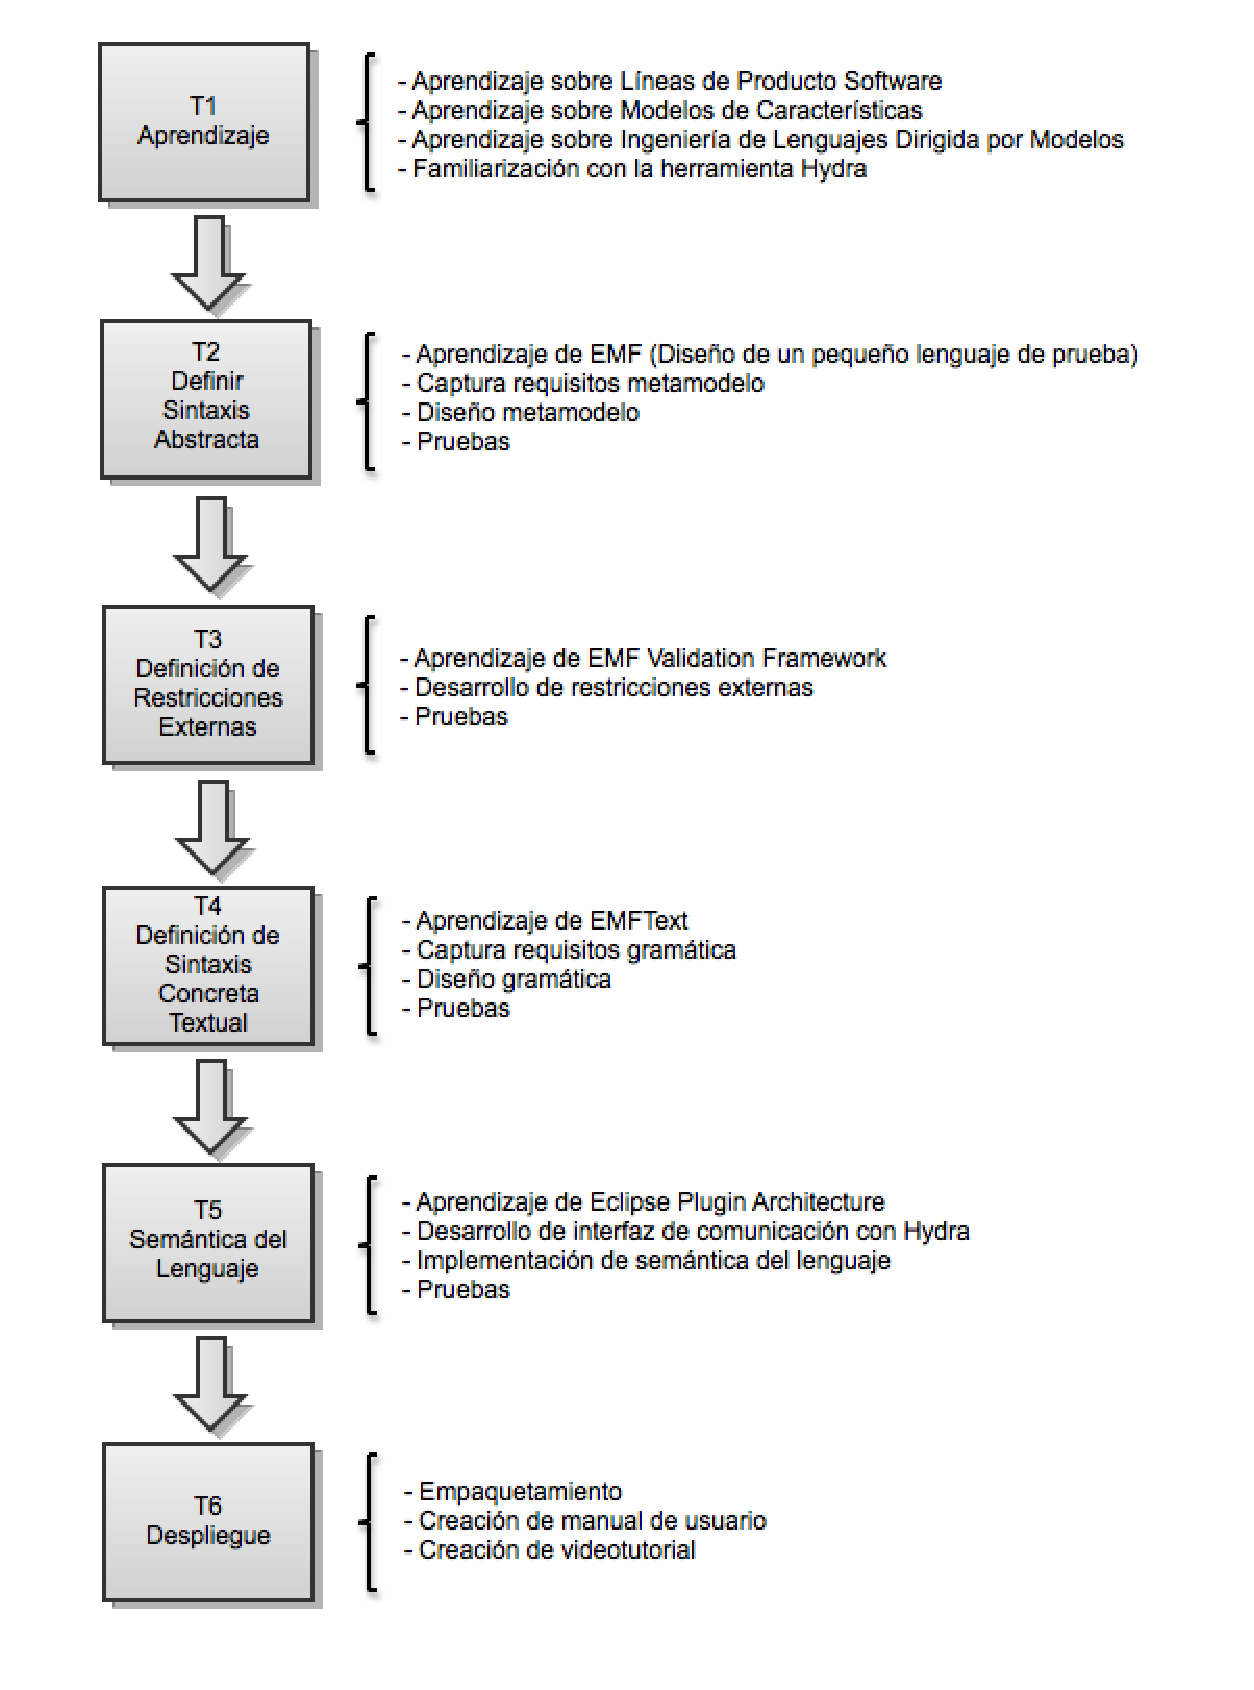
\includegraphics[scale=0.74]{planificacion/planning.eps}
    \caption{Proceso de desarrollo del Proyecto Fin de Carrera}
    \label{fig:planning}
\end{figure}

Obviamente, la primera tarea (Figura~\ref{fig:planning}-\emph{T1}) en este proceso de desarrollo fue la de adquirir los conocimientos necesarios para la realizaci�n de todas las tareas posteriores. Ello implicaba adquirir los conocimientos relacionados con las \emph{L�neas de Producto Software}~\cite{} en general y con los �rboles de caracter�sticas~\cite{} en particular, m�s concretamente, con la vesi�n de los �rboles de caracter�sticas que soportan la definici�n de caracter�sticas clonables~\cite{}. Dado que el proyecto se deb�a integrar con una herramienta para la especificaci�n y configuraci�n de �rboles de caracter�sticas concreta, denominada \emph{Hydra}~\cite{}, el siguiente paso fue el de familiarizarse con dicha herramienta y adquirir ciertos conocimientos sobre su arquitectura interna.

A continuaci�n, se tuvo que adquirir los conceptos necesarios para entender el funcionamiento de de la \emph{Ingenier�a de Lenguajes Dirigida por Modelos}~\cite{}. La familiarizaci�n con las tecnolog�as concretas relacionadas con la \emph{Ingenier�a de Lenguajes Dirigida por Modelos}, como la utilizaci�n de EMF (\emph{Eclipse Modelling Framework})~\cite{} para la definici�n de metamodelos, se realiz� dentro de cada fase concreto del proyecto, a medida que se iba necesitando aprender a utilizar dichas tecnolog�as.

%%========================================================================================%%
%% NOTA(Pablo): No pongas los tiempos que te ha costado cada tarea. Normalmente, no
%%              interesa y da mala imagen
%%========================================================================================%%

Tras esta tarea inicial de adquisici�n de conocimientos previos, el resto del proyecto se estructura como un proyecto de desarrollo de un lenguaje software siguiendo un enfoque dirigido por modelos. Consecuentemente, la primera tarea tras la fase inicial de documentaci�n (Figura~\ref{fig:planning}-\emph{T2}) fue la definici�n de la sintaxis abstracta, por medio de un metamodelo m�s un conjunto de restricciones externas, para el lenguaje que deb�a soportar nuestro editor. Para ello tuvimos que capturar los requisitos que deb�a satisfacer dicho lenguaje. Tras recoger dichos requisitos, se procedi� al dise�o del metamodelo y a la relizaci�n de las pruebas pertinentes con vistas a comprobar su correcto funcionamiento. Para crear dicho metamodelo se utiliz� el lenguaje de metamodelado Ecore, integrado dentro de la herramienta EMF (Eclipse Modelling Framework)~\cite{}.

A continuaci�n, de acuerdo con los expuesto en la secci�n anterior, procedimos a definir la las restricciones externas que no pod�an ser definidas en Ecore (Figura~\ref{fig:planning}-\emph{T3}). Dichas restricciones se implementaron utilizando la facilidad de EMF denominada EMF Validation Framework~\cite{}.

A continuaci�n, procedimos a definir la sintaxis concreta, en nuestro caso textual, para nuestro lenguaje de modelado. Optamos por una sintaxis textual ya que las restricciones a especificar son una especie de f�rmulas l�gicas, las cuales resultan m�s c�modas de especificar mediante notaciones textuales que mediante notaciones gr�ficas (Figura~\ref{fig:planning}-\emph{T4}). Para el desarrollo de dicha sintaxis textual hubo que hacer un nuevo an�lisis de los requisitos que dicha notaci�n textual deb�a satisfacer. A continuaci�n se especific� la gram�tica de nuestra sintaxis textual, ligando sus elementos con los del metamodelo producido en la fase anterior y se ejecutaron los casos de prueba necesarios para comprobar su correcto funcionamiento. Para crear dicha sintaxis textual se utiliz� la herramienta EMFText~\cite{}.

Las etapas anteriores permit�an disponer de un editor que soportaba la especificaci�n de restricciones de acuerdo al lenguaje HCL. Por tanto, s�lo restaba poder comprobar, para una configuraci�n dada de un �rbol de caracter�sticas, que dichas restricciones se satisfac�an. Ello implicaba dotar de sem�ntica al lenguaje y, a partir de dicha sem�ntica, implementar los mecanismos necesarios para la comprobaci�n de la validez de dichas restricciones. La sem�ntica del lenguaje ya estaba definida por el profesor Pablo S�nchez, por lo que s�lo hubo que implementar el c�digo necesario para procesar un modelo de restricciones y comprobar que dichas restricciones se satisfac�an. Dicho c�digo se implement� en Java, utilizando las facilidades que el entorno EMF proporciona para la manipulaci�n del modelo  (Figura~\ref{fig:planning}-\emph{T5}). Para poder implementar la sem�ntica, fue necesario crear una interfaz de comunicaci�n con la herramienta \emph{Hydra} que permitiese conocer el estado en el cual se hallaba cada caracter�stica. Tras la implementaci�n, se ejecut� un exhaustivo conjunto de pruebas para comprobar el correcto funcionamiento del c�digo creado.

En este punto del proceso de desarrollo ten�amos implementado el editor requerido, por lo que s�lo restaba proceder a su despliegue (Figura~\ref{fig:planning}-\emph{T6}). Este despliegue implicaba su integraci�n dentro de la arquitectura de plugins de Eclipse y, m�s concretamente, de la herramienta \emph{Hydra}. Tras dicha integraci�n, se procedi� a realizar una serie de pruebas de aceptaci�n, destinadas a comprobar que el trabajo realizado satisfac�a las necesidades de los usuarios finales que iban a utilizar el editor creado.



\section{Estructura del Documento}
\label{sec:intr:estructura}

% %%==================================================================%%
%% Author : Tejedo Gonz�lez, Daniel                                 %%
%%          S�nchez Barreiro, Pablo                                 %%
%% Version: 1.0, 22/11/2012                                         %%
%% Version: 2.0, 31/01/2013                                         %%
%%                                                                  %%
%% Memoria del Proyecto Fin de Carrera                              %%
%% Planificacion, planificacion                                     %%
%%==================================================================%%

Como se ha comentado con anterioridad, el objetivo de este Proyecto Fin de Carrera es el desarrollo de un editor para un novedoso lenguaje de especificaci�n y validaci�n de restricciones para �rboles de caracter�sticas donde dichas restricciones puedan incluir caracter�sticas clonables. Dicho editor se desarrollar� utilizando un moderno enfoque de \emph{Ingenier�a de Lenguajes Dirigido por Modelos}. Por tanto, el proceso de desarrollo del presente proyecto queda pr�cticamente determinado por dicho enfoque, el cual posee un proceso de desarrollo bien definido, el cual se describi� en la secci�n anterior. La Figura~\ref{fig:planning} muestra como dicho proceso de desarrollo se ha instanciado para nuestro caso particular.

%%==================================================================%%
%% NOTA(Pablo): En esta imagen hay que hacer cambios                %%
%%              Te los indico de foma verbal cuando pases por el    %%
%%              despacho, pero hay que mejorar su consistencia      %%
%%==================================================================%%

\begin{figure}[!tb]
    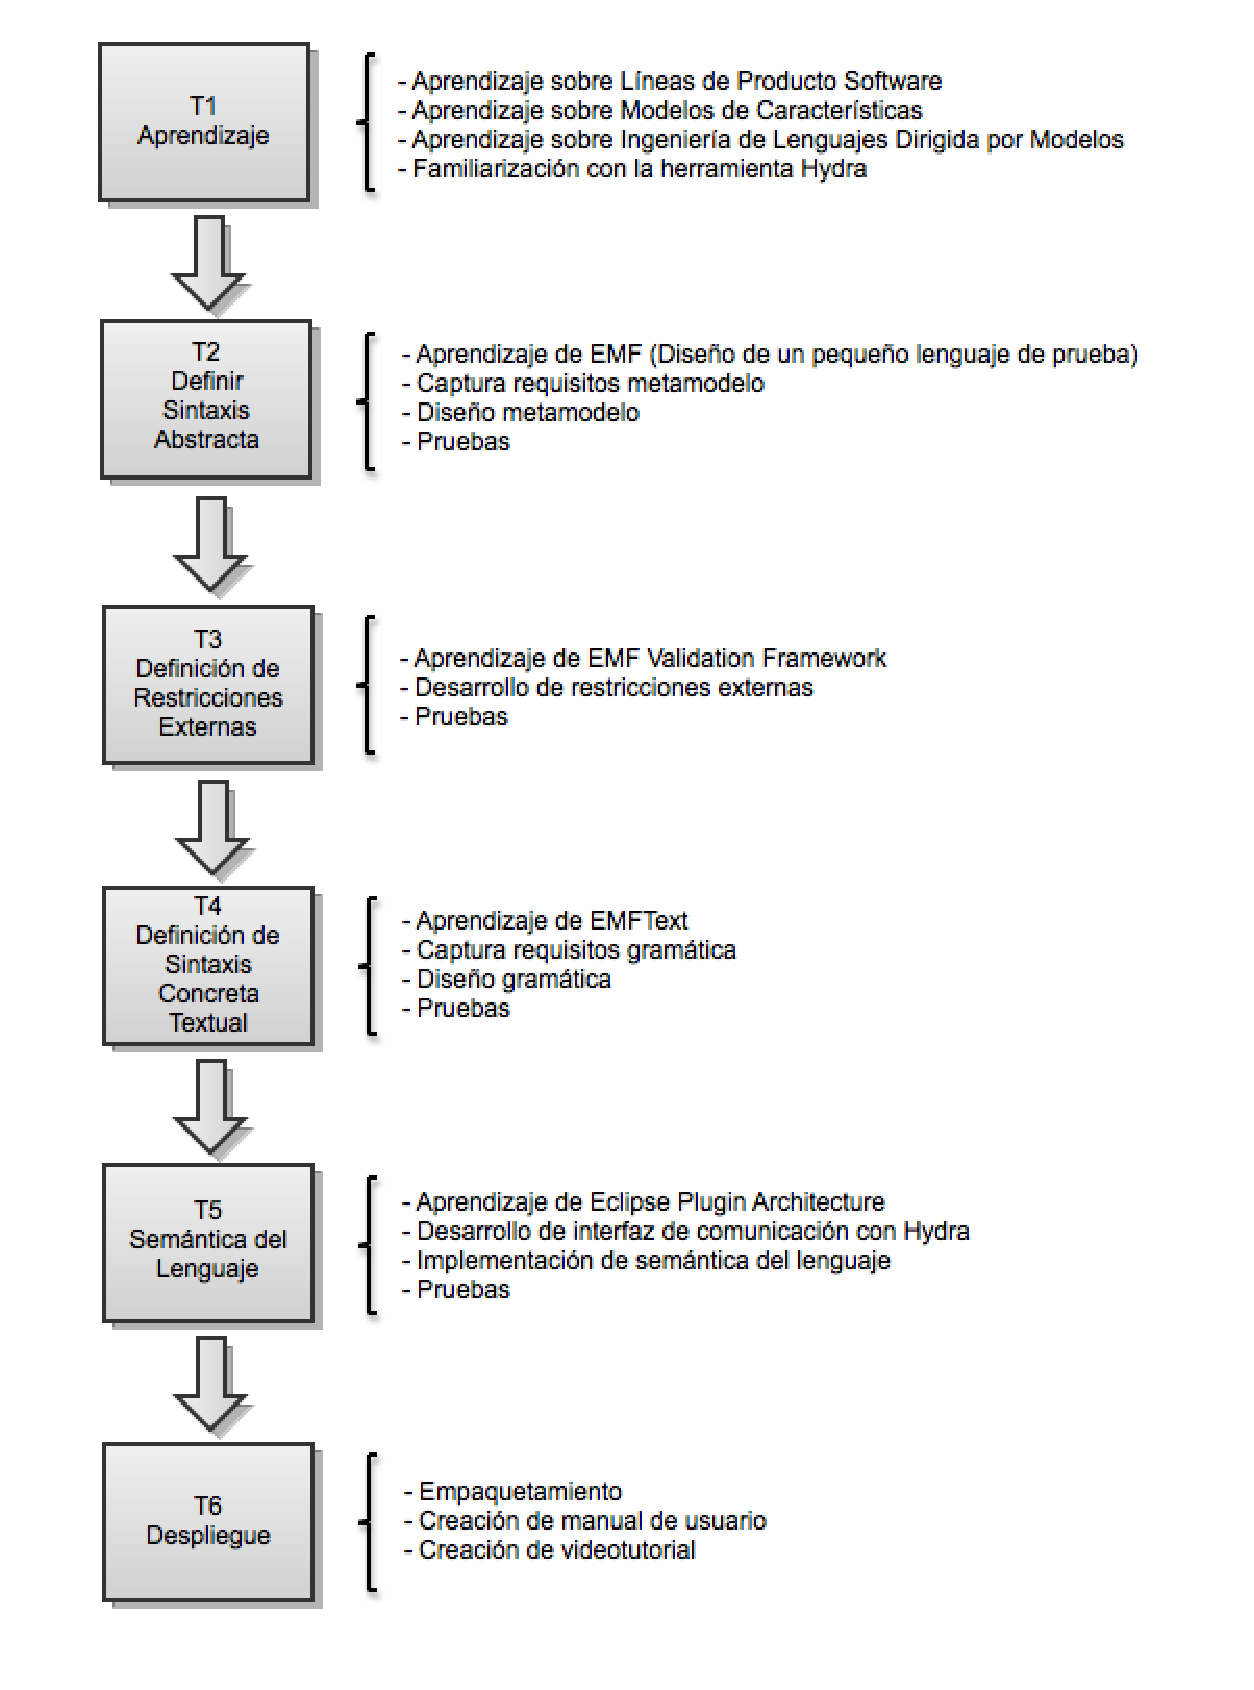
\includegraphics[scale=0.74]{planificacion/planning.eps}
    \caption{Proceso de desarrollo del Proyecto Fin de Carrera}
    \label{fig:planning}
\end{figure}

Obviamente, la primera tarea (Figura~\ref{fig:planning}-\emph{T1}) en este proceso de desarrollo fue la de adquirir los conocimientos necesarios para la realizaci�n de todas las tareas posteriores. Ello implicaba adquirir los conocimientos relacionados con las \emph{L�neas de Producto Software}~\cite{} en general y con los �rboles de caracter�sticas~\cite{} en particular, m�s concretamente, con la vesi�n de los �rboles de caracter�sticas que soportan la definici�n de caracter�sticas clonables~\cite{}. Dado que el proyecto se deb�a integrar con una herramienta para la especificaci�n y configuraci�n de �rboles de caracter�sticas concreta, denominada \emph{Hydra}~\cite{}, el siguiente paso fue el de familiarizarse con dicha herramienta y adquirir ciertos conocimientos sobre su arquitectura interna.

A continuaci�n, se tuvo que adquirir los conceptos necesarios para entender el funcionamiento de de la \emph{Ingenier�a de Lenguajes Dirigida por Modelos}~\cite{}. La familiarizaci�n con las tecnolog�as concretas relacionadas con la \emph{Ingenier�a de Lenguajes Dirigida por Modelos}, como la utilizaci�n de EMF (\emph{Eclipse Modelling Framework})~\cite{} para la definici�n de metamodelos, se realiz� dentro de cada fase concreto del proyecto, a medida que se iba necesitando aprender a utilizar dichas tecnolog�as.

%%========================================================================================%%
%% NOTA(Pablo): No pongas los tiempos que te ha costado cada tarea. Normalmente, no
%%              interesa y da mala imagen
%%========================================================================================%%

Tras esta tarea inicial de adquisici�n de conocimientos previos, el resto del proyecto se estructura como un proyecto de desarrollo de un lenguaje software siguiendo un enfoque dirigido por modelos. Consecuentemente, la primera tarea tras la fase inicial de documentaci�n (Figura~\ref{fig:planning}-\emph{T2}) fue la definici�n de la sintaxis abstracta, por medio de un metamodelo m�s un conjunto de restricciones externas, para el lenguaje que deb�a soportar nuestro editor. Para ello tuvimos que capturar los requisitos que deb�a satisfacer dicho lenguaje. Tras recoger dichos requisitos, se procedi� al dise�o del metamodelo y a la relizaci�n de las pruebas pertinentes con vistas a comprobar su correcto funcionamiento. Para crear dicho metamodelo se utiliz� el lenguaje de metamodelado Ecore, integrado dentro de la herramienta EMF (Eclipse Modelling Framework)~\cite{}.

A continuaci�n, de acuerdo con los expuesto en la secci�n anterior, procedimos a definir la las restricciones externas que no pod�an ser definidas en Ecore (Figura~\ref{fig:planning}-\emph{T3}). Dichas restricciones se implementaron utilizando la facilidad de EMF denominada EMF Validation Framework~\cite{}.

A continuaci�n, procedimos a definir la sintaxis concreta, en nuestro caso textual, para nuestro lenguaje de modelado. Optamos por una sintaxis textual ya que las restricciones a especificar son una especie de f�rmulas l�gicas, las cuales resultan m�s c�modas de especificar mediante notaciones textuales que mediante notaciones gr�ficas (Figura~\ref{fig:planning}-\emph{T4}). Para el desarrollo de dicha sintaxis textual hubo que hacer un nuevo an�lisis de los requisitos que dicha notaci�n textual deb�a satisfacer. A continuaci�n se especific� la gram�tica de nuestra sintaxis textual, ligando sus elementos con los del metamodelo producido en la fase anterior y se ejecutaron los casos de prueba necesarios para comprobar su correcto funcionamiento. Para crear dicha sintaxis textual se utiliz� la herramienta EMFText~\cite{}.

Las etapas anteriores permit�an disponer de un editor que soportaba la especificaci�n de restricciones de acuerdo al lenguaje HCL. Por tanto, s�lo restaba poder comprobar, para una configuraci�n dada de un �rbol de caracter�sticas, que dichas restricciones se satisfac�an. Ello implicaba dotar de sem�ntica al lenguaje y, a partir de dicha sem�ntica, implementar los mecanismos necesarios para la comprobaci�n de la validez de dichas restricciones. La sem�ntica del lenguaje ya estaba definida por el profesor Pablo S�nchez, por lo que s�lo hubo que implementar el c�digo necesario para procesar un modelo de restricciones y comprobar que dichas restricciones se satisfac�an. Dicho c�digo se implement� en Java, utilizando las facilidades que el entorno EMF proporciona para la manipulaci�n del modelo  (Figura~\ref{fig:planning}-\emph{T5}). Para poder implementar la sem�ntica, fue necesario crear una interfaz de comunicaci�n con la herramienta \emph{Hydra} que permitiese conocer el estado en el cual se hallaba cada caracter�stica. Tras la implementaci�n, se ejecut� un exhaustivo conjunto de pruebas para comprobar el correcto funcionamiento del c�digo creado.

En este punto del proceso de desarrollo ten�amos implementado el editor requerido, por lo que s�lo restaba proceder a su despliegue (Figura~\ref{fig:planning}-\emph{T6}). Este despliegue implicaba su integraci�n dentro de la arquitectura de plugins de Eclipse y, m�s concretamente, de la herramienta \emph{Hydra}. Tras dicha integraci�n, se procedi� a realizar una serie de pruebas de aceptaci�n, destinadas a comprobar que el trabajo realizado satisfac�a las necesidades de los usuarios finales que iban a utilizar el editor creado.




 % Chapter 1

% Cap�tulo 2: Resumen del Estado del Arte
% %%==================================================================%%
%% Author : Sa�udo Olmedo, Ignacio                                  %%
%%          S�nchez Barreiro, Pablo                                 %%
%% Version: 1.3, 18/06/2014                                         %%
%%                                                                  %%
%% Memoria del Proyecto Fin de Carrera                              %%
%% Antecedentes, archivo ra�z                                       %%
%%==================================================================%%

\chapterheader{Antecedentes y Planificaci�n}{Antecedentes y Planificaci�n}
\label{chap:background}

Este cap�tulo describe las tecnolog�as y t�cnicas utilizadas en el desarrollo del presente Proyecto de Fin de Carrera. La primera secci�n est� dedicada a introducir el caso de estudio que se analizar� a lo largo del presente proyecto. La siguiente secci�n est� dedicada a describir en qu� consiste Eclipse Modeling Framework (EMF) la herramienta utilizada para desarrollar lenguajes de modelado. A continuaci�n se describe la herramienta Epsilon, herramienta que se ha utilizado para desarrollar el generador de c�digo. La siguiente secci�n est� dedicada a explicar de manera breve algunos conceptos de Cassandra. Finalmente se expone la planificaci�n que ha seguido el proyecto para su realizaci�n, desde formaci�n hasta etapas de desarrollo.

\chaptertoc

\section{Caso de estudio: Generador de c�digo CQL-Cassandra}
\label{sec:back:casoEstudio}

%%==========================================================================%%
%% Author : Sa�udo Olmedo, Ignacio                                          %%
%% Author : S�nchez Barreiro, Pablo                                         %%
%% Version: 1.2, 21/04/2014                                                 %%
%%                                                                          %%
%% Memoria del Proyecto Fin de Carrera                                      %%
%% M2M/Caso de estudio                                                      %%
%%==========================================================================%%

Como se explicaba en el capitulo 2 en la secci�n "Caso de estudio" el objetivo de este caso de estudio es la creaci�n de un generador de c�digo de una versi�n simplificada de Twitter.
En esta secci�n se reproducir�n los procesos M2M y M2T en el siguiente capitulo, todo esto bajo el proceso de desarrollo dirigido por modelos. Esta secci�n esta dedicada a describir la transformaci�n del modelo UML de Twissandra a un modelo Cassandra. Partiendo del modelo UML de la figura~\ref{back:fig:twissandra} y una vez establecidas las reglas de transformaci�n entre modelos, esta secci�n explica el proceso de transformaci�n del modelo UML al modelo Cassandra.

En primer lugar, marcamos el atributo username de la clase User como clave. En el caso de la clase FollowingRelationship y la clase Tweet al no tener un atributo marcado como clave generamos una clave sustituta autom�ticamente para cada clase, llamadas FollowingRelationship\_id y tweet\_id respectivamente.

Por cada paquete estereotipado como <<dataModel>>, se crea un nuevo keyspace. El nombre del keyspace ser� el nombre utilizado por el data model. Los atributos restantes de las meta-clases del keyspace se establecen en sus valores definidos por defecto. A continuaci�n, todos los elementos correspondientes de ese paquete se procesan y se colocan dentro de su keyspace correspondiente.

Como se mencionaba en las reglas de transformaci�n, la clase User se transforma en una Column Family llamada User. A continuaci�n, los atributos y las asociaciones se procesan. Por �ltimo, el atributo Username, que se marc� como clave en el modelo de datos UML, es marcado como Primary Key. De manera similar para aquellos atributos del modelo UML cuya multiplicidad sea igual a uno se realiza una transformaci�n simple, por ejemplo el atributo username y password se transforman en dos columnas, ambos del tipo text. Estas columnas est�n contenidas en la column family User. De la misma manera se transforman los atributos body y time de la clase Tweet y el atributo timestamp de la clase FollowingRelationship.
En el caso de el atributo del modelo UML email cuya multiplicidad es mayor de uno y tiene las propiedades isUnique establecida en false y la propiedad isOrdered establecida en false (en el modelo no se puede apreciar pero esta configurado as�), se transforma este atributo en un set llamado email de tipo text dentro de la column family User.

En cuanto a las asociaciaciones de multiplicidad igual a uno la transformaci�n que se realiza por ejemplo, para la asociaci�n de la clase user una nueva columna llamada user\_username (recordemos que username es la clave de la column family user) es creada y a�adida a la column family Tweet. Para las asociaciones cuya multiplicidad es mayor de uno, por ejemplo la asociaci�n llamada userline se crea una dynamic column family llamada User\_userline. A continuaci�n una columna llamada user\_username de tipo text es a�adida a esta column family. Despu�s una columna llamada tweet\_id de tipo uuid es a�adida (el atributo tweet\_id fue creado en la column family tweet al no tener clave). Las columnas user\_username y tweet\_id son designadas como primary key, la columna user\_username ser� la partition key. 

\section{EMF}
\label{sec:back:EMF}

%%==================================================================%%
%% Author : Sa�udo Olmedo, Ignacio                                  %%
%%          S�nchez Barreiro, Pablo                                 %%
%% Version: 1.3, 18/06/2014                                         %%
%%                                                                  %%
%% Memoria del Proyecto Fin de Carrera                              %%
%% Background/EMF                                                   %%
%===================================================================%%
Para comenzar el desarrollo del proyecto bajo el paradigma del desarrollo software dirigido por modelos necesitamos definir que lenguajes de modelado vamos a utilizar. En el cap�tulo anterior coment�bamos que es necesario definir el lenguaje de modelado que utilizara Cassandra para ello usaremos EMF. Eclipse Modeling Framework (EMF) (\cite{dave:2008}) es un framework de modelado que nos proporciona la base para la elaboraci�n de lenguajes de modelado. Para la creaci�n de meta-modelos EMF (\cite{kolovos:2014}) utiliza dos modelos de meta-datos: \emph{Ecore} y \emph{Genmodel}. Ecore contiene la informaci�n sobre las clases que se han definido. Genmodel contiene informaci�n adicional para la generaci�n del c�digo, por ejemplo la ruta y la informaci�n del archivo. Genmodel tambi�n contiene atributos que sirven de control a la hora de generar el c�digo, encontramos los siguientes par�metros de control:
\begin{enumerate}
\item EClass: representa una clase, con cero o m�s atributos y cero o m�s referencias.
\item EAttribute: representa un atributo que tiene un nombre y un tipo.
\item EReference: representa un extremo de una asociaci�n entre dos clases.
\item EDataType: representa el tipo de un atributo, por ejemplo, int, float.
\end{enumerate}
Estos atributos nos servir�n a la hora de crear las reglas de transformaci�n entre modelos UML y modelos Cassandra.

Utilizando EMF se pueden crear meta-modelos de forma gr�fica muy similar a los diagramas de clases en UML.
EMF permite crear un meta-modelo a trav�s de diferentes medios, por ejemplo, XMI, anotaciones Java, XML o UML. Adem�s EMF proporciona un framework para almacenar la informaci�n del modelo.
Un ejemplo sencillo de la utilidad de EMF es el siguiente: Imaginemos que deseamos construir una aplicaci�n para manipular mensajes escritos en XML. El primer paso que dar�amos ser�a empezar definiendo el schema del mensaje sin embargo con EMF se puede trabajar ignorando este nivel. Con EMF podemos crear plugins que generen por ejemplo un diagrama de clases UML a partir de este mensaje XML o directamente generar el c�digo Java que implemente las clases del mensaje XML.




\section{Epsilon}
\label{sec:back:epsilon}

%%==================================================================%%
%% Author : Sa�udo Olmedo, Ignacio                                  %%
%%          S�nchez Barreiro, Pablo                                 %%
%% Version: 1.1, 18/06/2014                                         %%
%%                                                                  %%
%% Memoria del Proyecto Fin de Carrera                              %%
%% Background/Epsilon                                               %%
%===================================================================%%


Epsilon es una familia de lenguajes y herramientas para el desarrollo de software dirigido por modelos, entre estas herramientas podemos encontrar: herramientas de transformaci�n de modelos, validaci�n de modelos o generaci�n de c�digo entre otras funcionalidades. Epsilon es distribuido a trav�s de la plataforma de modelado de lenguajes de Eclipse.
Epsilon proporciona multitud de lenguajes y herramientas para trabajar con modelos. Los lenguajes utilizados en este proyecto son \emph{EOL} (Epsilon Object Language), \emph{ETL} (Epsilon Transformation Language) y \emph{EGL} (Epsilon Generation Language) tambi�n ha sido utilizado \emph{EUnit} como herramienta para validar el c�digo escrito por el generador de c�digo Cassandra-CQL. Estos lenguajes y herramientas son descritos a continuaci�n. Toda la informaci�n sobre estos lenguajes as� como su utilizaci�n ha sido obtenida de (\cite{kolovos:2014})

\subsection{Epsilon Object Language}
\emph{Epsilon Object Language} (EOL) es un lenguaje de programaci�n imperativo utilizado para crear, consultar y modificar los modelos EMF. EOL se puede considerar un lenguaje mezcla de Javascript y OCL, que combina lo mejor de ambos lenguajes. Como tal, proporciona todas las caracter�sticas habituales imperativas que se encuentran en Javascript (por ejemplo, la secuencia de la declaraci�n, las variables, bucles for y while, etc) y todas las caracter�sticas interesantes de OCL como las operaciones sobre colecciones, por ejemplo Sequence\{1..5\}.select(x \textbar\ x \textgreater\ 3).


\begin{figure}[!tb]
  \centering
  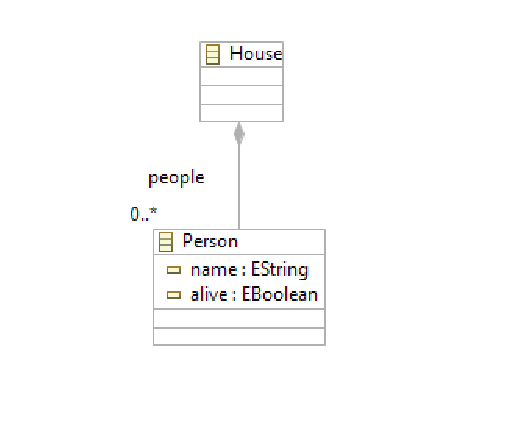
\includegraphics[width=.8\linewidth]{background/images/ejCasa.eps} \\
  \caption{Ejemplo metamodelo casa}
  \label{back:fig:ejMetamodeloCasa}
\end{figure}


Para entender mejor el funcionamiento de EOL se expone el siguiente ejemplo. Se ha definido el meta-modelo mostrado en la figura~\ref{back:fig:ejMetamodeloCasa}, este meta-modelo consiste en la representaci�n de una casa y las personas que viven en ella. Las personas tienen un nombre y un atributo booleano que representa si una persona est� viva o no. Existe una relaci�n de agregaci�n para reflejar que la casa contiene personas.
Una vez creado el meta-modelo podemos crear un modelo como instancia de ese meta-modelo. Un ejemplo de c�mo funciona EOL puede ser el siguiente: deseamos saber que personas habitan en la casa y est�n vivas. La sintaxis correspondiente ser�a la siguiente (figura~\ref{back:code:codigoEOL}).

\begin{figure}[!tb]
\begin{center}
\begin{footnotesize}
\begin{verbatim}
--------------------------------------------------------
for (person in Person.all){
  if (person.alive == true) {
    person.name.println();
  }
}

//Podemos realizar lo mismo de la siguiente manera:

Person.all.select(r|r.alive==true).name.println();

--------------------------------------------------------
\end{verbatim}
\end{footnotesize}
\end{center}
\caption{Ejemplo c�digo EOL}
\label{back:code:codigoEOL}
\end{figure}


Como vemos la sintaxis es muy similar a cualquier lenguaje orientado a objetos, podemos manipular y consultar los objetos del modelo, sin embargo EOL no nos permite la definici�n de clases.


\subsection{Epsilon Transformation Language}
\emph{Epsilon Transformation Language} (ETL) es un lenguaje de transformaci�n modelo a modelo basado en reglas (\imp{Model to Model-M2M}). ETL proporciona las caracter�sticas est�ndar de un lenguaje de transformaci�n, tambi�n nos permite manipular los modelos de entrada y salida as� como su c�digo fuente. ETL tiene su propia sintaxis sin embargo utiliza el lenguaje EOL como base.


Recordando el ejemplo de la Red de computadores y el Grafo detallado en el capitulo anterior (secci�n 1.2). Deseamos realizar la transformaci�n de un modelo de tipo grafo a un modelo de tipo red para ello definiremos una serie de reglas de transformaci�n utilizando para ello ETL. En primer lugar necesitamos definir el modelo del grafo para poder realizar la transformaci�n a un modelo de tipo Red.
La figura~\ref{back:code:codigoETL} muestra el c�digo que realiza el proceso de transformaci�n de un Grafo a una Red.

\begin{figure}[!tb]
\begin{center}
\begin{footnotesize}
\begin{verbatim}

rule Arista2Cable
transform a : Grafo!Arista
to r : Red!Cable {	
    r.nameCable = a.nombreArista;
    if (a.parent.isDefined()) {
        r.parent=Red;
        for (nodoArista in a.children) {
            if(nodoArista.color=TColor#R){
                var PC : new Red!PC;
                PC.nameNodo="PC"+iPC;
                r.children.add(PC);
                iPC=iPC+1;	
            }
            else{
                var Router : new Red!Router;
                Router.nameNodo="Router"+iRouter;
                r.children.add(Router);
                iRouter=iRouter+1;
            }
        }
    }	
}

\end{verbatim}
\end{footnotesize}
\end{center}
\caption{Ejemplo c�digo ETL}
\label{back:code:codigoETL}
\end{figure}

En este c�digo encontramos solo una regla. Esta regla transforma aristas del grafo a cables de la red. La primera instrucci�n copia el nombre de la arista al cable. A continuaci�n la primera condicional cuestiona si esa arista tiene un padre definido en caso afirmativo asigna el cable a la red. A continuaci�n por cada nodo se crea o bien un PC o un router dependiendo del color del nodo que se est� analizando (rojo-PC, azul-Router). En siguiente lugar se asigna el nodo creado al cable correspondiente y finalmente se a�ade a la red. Este proceso se repite por cada arista del grafo. Una vez ejecutado este c�digo dado un modelo de entrada de tipo Grafo obtenemos un modelo equivalente de tipo Red que cumple las reglas definidas en el meta-modelo.


\subsection{Epsilon Generation Language}

\emph{Epsilon Generation Language} (EGL) (\cite{louis:2008}) es un lenguaje utilizado para la generaci�n de c�digo basado en la transformaci�n de modelos (\imp{Model to Text-M2T}).
EGL puede ser utilizado para transformar modelos en cualquier tipo de lenguaje, por ejemplo c�digo ejecutable Java, c�digo HTML o incluso aplicaciones completas que comprenden el c�digo en varios lenguajes (por ejemplo, HTML, Javascript y CSS). En este proyecto se utilizara EGL para la generaci�n de c�digo Cassandra Query Language (CQL) a partir de modelos UML 2.0.

Cada plantilla de EGL contiene varias secciones. Cada secci�n puede ser est�tica o bien din�mica.
Una secci�n est�tica contiene texto que aparecer� en la salida generada por la plantilla. Una secci�n din�mica comienza con la secuencia '[\%' y termina con la secuencia '\%]'. La secci�n din�mica contiene lenguaje EOL.
La figura~\ref{back:code:codigoEGL} muestra como se realiza la generaci�n de c�digo HTML utilizando para ello el modelo generado de una red a partir de un grafo (ver secci�n anterior).

\begin{figure}[!tb]
\begin{center}
\begin{footnotesize}
\begin{verbatim}
--------------------------------------------------------
[%
    var red: Red := Red.allInstances().at(0);
%]

<html>
    <head>
        <title> Red </title>
    </head>
    <body>
        <h1>Conexiones</h1>				
        <table  border="1">
            <col style="width: 200px" />
            <col style="width: 100px" span="3" />
            [% for (conexiones in red.conexiones){%]
            <tr>
                <th scope="row">[%=conexiones.nameCable%]</th>
                [% for (nodos in conexiones.children){%]
                    <td>[%=nodos.nameNodo%]</td>
                [%	}%]
            </tr>
            [%	}%]
        </table>
    </body>
</html>
--------------------------------------------------------
\end{verbatim}
\end{footnotesize}
\end{center}
\caption{Ejemplo c�digo EGL}
\label{back:code:codigoEGL}
\end{figure}

Como vemos en el c�digo la integraci�n del c�digo EGL junto con HTML es total, en este sencillo c�digo se genera una p�gina HTML con una tabla que muestra varias filas, una fila por cada conexi�n entre dos componentes de la red. 

\section{Cassandra}
\label{sec:back:cassandra}

%%==================================================================%%
%% Author : Sa�udo Olmedo, Ignacio                                  %%
%%          S�nchez Barreiro, Pablo                                 %%
%% Version: 1.1, 18/06/2014                                         %%
%%                                                                  %%
%% Memoria del Proyecto Fin de Carrera                              %%
%% Background/Cassandra                                             %%
%===================================================================%%
http://www.nosql-database.org/
[chalmers]
%http://www.acens.com/wp-content/images/2014/02/bbdd-nosql-wp-acens.pdf
%http://www.strozzi.it/cgi-bin/CSA/tw7/I/en_US/NoSQL/Philosophy%20of%20NoSQL
Desde que naci� SQL en el a�o 1974, SQL ha sido el modelo de base de datos relacionales utilizado por excelencia. En los �ltimos a�os ha surgido otra vertiente denominada NoSQL la cual surge por la necesidad de manejo de grandes vol�menes de informaci�n no estructurada, distribuida con la mayor rapidez posible. NoSQL es usado en plataformas como Facebook o Twitter. Podemos encontrar varios tipos de bases de datos no relacionales; Bases de datos documentales, bases de datos clave-valor, orientadas a grafos y mas tipos.

Las principales caracter�sticas de NoSQL que difieren de SQL son:
\begin{enumerate}
\item NoSQL no garantiza las propiedades ACID (atomicidad, coherencia, aislamiento y durabilidad).
\item No utiliza SQL como lenguaje de consultas. Algunas bases de datos no relacionales utilizan SQL como lenguaje de apoyo sin embargo la mayor�a utilizan su propio lenguaje de consultas como por ejemplo Cassandra que utiliza CQL.
\item No est� permitido el uso de joins ya que al manejar grandes vol�menes de informaci�n una consulta con un join puede llegar a sobrecargar el sistema.
\item Escalan horizontalmente y trabajan de manera distribuida por lo que la informaci�n puede estar en distintas maquinas y el a�adir nodos mejora el rendimiento.
\item Resuelven problemas de altos vol�menes de informaci�n
\end{enumerate}

En este proyecto de fin de carrera se utiliza Cassandra, Cassandra es una distribuci�n de bases de datos no relaciones (NoSQL). Dentro del mundo de las bases de datos no relaciones Cassandra pertenece a la familia de bases de datos denominada "clave-valor". Las bases de datos clave-valor son aquellas que  asocian los valores a una determinada clave esto permite la recuperaci�n y escritura de informaci�n de forma muy r�pida y eficiente. Cassandra re�ne las  tecnolog�as de sistemas distribuidos de Amazon Dynamo y el modelo de datos BigTable de Google. Al igual que Dynamo, Cassandra es consistente. Como BigTable, Cassandra proporciona un modelo de datos basado en ColumnFamily siendo considerado el sistema basado en clave-valor m�s popular.

Las bases de datos basadas en Cassandra son soluciones utilizadas cuando es necesaria escalabilidad y alta disponibilidad sin comprometer el rendimiento. Escalabilidad lineal y tolerancia a fallos o infraestructura en la nube lo convierten en la plataforma perfecta para datos de misi�n critica. Cassandra proporciona gran estabilidad en cuanto a la replicaci�n de datos a trav�s de m�ltiples datacenters, consiguiendo una menor latencia para sus usuarios y la tranquilidad de que no existan perdidas de datos ante ca�das. Cassandra utiliza un lenguaje llamado CQL (Cassandra Query Language) con una sintaxis muy similar a SQL aunque con menos funcionalidades.

Fue dise�ado por Avinash Lakshman (uno de los creadores de Amazon's Dynamo) y Prashant Malik (Ingeniero de Facebook). Cassandra est� en producci�n para Facebook sin embargo aun est� en fase de desarrollo.

%https://cassandra.apache.org/ http://www.datastax.com/documentation/cql/3.0/cql/ddl/ddl_intro_c.html

A continuaci�n se explican algunos t�rminos que hay que tener en cuenta cuando se trabaja con Cassandra.
En Cassandra un KeySpace es el equivalente a una base de datos en los sistemas de bases de datos relacionales. El conocido t�rmino de tabla en las bases de datos relacionales tiene su equivalente en Cassandra llamado Column Family. Por lo tanto un KeySpace puede contener varias Column Families y una Column Family a su vez contiene varias columnas.
Una columna es la unidad de almacenamiento b�sica, est� formada de tres campos: Nombre, un valor y un timestamp. El nombre y el valor se almacena como una matriz de bytes sin procesar y pueden ser de cualquier tama�o. Un ejemplo:
Nombre de la columna 	\"Username\"
Nombre de usuario	\"Ignacio\"
Timestamp 		\"123456789\"
La sintaxis del lenguaje CQL es muy similar a SQL, CQL contiene sintaxis ya conocida de SQL como INSERT, DELETE, UPDATE, INSERT,  ...
Un ejemplo de c�digo CQL ejecutable es el siguiente (Figura~\ref{back:code:codigoCQL})


\begin{figure}[!tb]
\begin{center}
\begin{footnotesize}
\begin{verbatim}

DROP KEYSPACE twitter;

CREATE KEYSPACE twitter
WITH replication = {'class':'SimpleStrategy', 'replication_factor':2};

USE twitter;

CREATE TABLE Tweet(
       UUID text,
       usernameTw text,
       body text,
       PRIMARY KEY(UUID)
);

CREATE TABLE User(
       username text,
       password text,
       followers set<text>,
       followings set<text>,
       tweets_written list<text>,
       PRIMARY KEY(username)
);

\end{verbatim}
\end{footnotesize}
\end{center}
\caption{Ejemplo c�digo CQL}
\label{back:code:codigoCQL}
\end{figure}




\section{Planificaci�n}
\label{sec:back:planificacion}

%%==================================================================%%
%% Author : Sa�udo Olmedo, Ignacio                                  %%
%%          S�nchez Barreiro, Pablo                                 %%
%% Version: 1.2, 18/06/2013                                         %%
%%                                                                  %%
%% Memoria del Proyecto Fin de Carrera                              %%
%% Background/Planificacion                                         %%
%===================================================================%%

El objetivo de este proyecto de fin de carrera es la implementaci�n de un generador de c�digo Cassandra a partir de modelos UML. El proceso de desarrollo as� como el de aprendizaje que se ha seguido para la realizaci�n del proyecto es descrito a continuaci�n.

La primera tarea como es evidente consisti� en adquirir los conocimientos necesarios para el desarrollo del proyecto, en primer lugar todo lo relacionado con el proceso de modelado de un lenguaje y transformaci�n de lenguajes [kleppe]. Tambi�n fueron necesarios conocimientos sobre la Ingenier�a y el Desarrollo Dirigido por Modelos, as� como de la sintaxis, arquitectura y funcionamiento de Cassandra.

A continuaci�n se comenz� a trabajar con la herramienta Epsilon, sus lenguajes EOL, EGL, ETL y EUnit como herramienta para las pruebas de los modelos y c�digo generados. As� como con el lenguaje para la definici�n de lenguajes de modelado Eclipse Modeling Framework (EMF).
Para conocer c�mo funcionaban estos lenguajes se desarrollaron una serie de casos pr�cticos para familiarizarse con los m�todos de transformaci�n as� como con la herramienta, para ello se realizo el proceso completo para crear un generador de c�digo desde la transformaci�n entre modelos hasta la transformaci�n modelo-c�digo. Estos casos de prueba son los que se exponen en la secci�n de Epsilon.

Una vez conocido estos conceptos se estudiaron las reglas de transformaci�n a aplicar para transformar un modelo UML a un modelo Cassandra, estas reglas fueron propuestas por [pabloCassandra].

Tras estas tareas de adquisici�n de conocimientos se empez� a trabajar en el generador de c�digo Cassandra empezando por la transformaci�n de modelos UML a modelos Cassandra. Estas transformaciones son expuestas en el siguiente cap�tulo. Una vez finalizada la transformaci�n se comenz� a trabajar en el generador de c�digo Cassandra, esta tarea es descrita en el cap�tulo 5. Tras realizar dicha tarea se realizaron una serie de casos de prueba para verificar si los resultados que otorgaba el generador de c�digo eran los esperados, para esta tarea utilizamos la herramienta EUnit.

Finalmente y tras generar varios casos de ejemplo se instalo la plataforma de Cassandra BLABLA 

\section{Sumario}
\label{sec:back:sumario}

%%==================================================================%%
%% Author : Abascal Fern�ndez, Patricia                             %%
%%          S�nchez Barreiro, Pablo                                 %%
%% Version: 1.1, 21/06/2013                                         %%
%%                                                                  %%
%% Memoria del Proyecto Fin de Carrera                              %%
%% Antecedentes, Sumario                                            %%
%%==================================================================%%

Durante este cap�tulo se han descrito los conceptos necesarios para comprender el �mbito y el alcance de este proyecto. Se ha descrito el caso de estudio que se utilizar� a lo largo del documento. A continuaci�n, se ha especificado qu� es una l�nea de productos software, el dise�o orientado a caracter�sticas, la metodolog�a TENTE, las limitaciones de las clases parciales en C\#, c�mo pueden resolverse estas limitaciones mediante el uso del \emph{SlicerPattern} y el proceso de generaci�n de c�digo con Epsilon.



% Cap�tulo 3: Domain Engineering
% %%==================================================================%%
%% Author : Sa�udo Olmedo, Ignacio                                  %%
%% Author : S�nchez Barreiro, Pablo                                 %%
%% Version: 1.1, 21/04/2014                                         %%
%%                                                                  %%
%% Memoria del Proyecto Fin de Carrera                              %%
%% M2M, Archivo ra�z                                                %%
%%==================================================================%%

\chapterheader{Transformaci�n modelo a modelo}{Transformaci�n modelo a modelo}
\label{chap:m2m}

Este cap�tulo describe el primer paso de nuestro proceso de desarrollo, que la transformaci�n un modelo conceptual UML 2.0 a un modelo de una implementaci�n en Cassandra. Para ello, en primer lugar necesitamos un metamodelo de los modelos de implementaci�n Cassandra. En segundo lugar debemos definir las reglas de transformaci�n para convertir un modelo UML a un modelo en Cassandra. Por �ltimo, deberemos verificar mediante pruebas el correcto funcionamiento de las transformaciones implementadas.

\chaptertoc

\section{Introducci�n}
\label{domain:sec:intro}

%%==================================================================%%
%% Author : Abascal Fern�ndez, Patricia                             %%
%%          S�nchez Barreiro, Pablo                                 %%
%% Version: 1.0, 14/02/2013                                         %%                                                                                    %%                                                                  %%
%% Memoria del Proyecto Fin de Carrera                              %%
%% Archivo ra�z                                                     %%
%%==================================================================%%

\chapterheader{Introducci�n}{Introducci�n}
\label{chap:introduction}

Este cap�tulo sirve de introducci�n a la presente Memoria de Proyecto Fin de Carrera. En �l se describen los objetivos generales del proyecto, as� como el contexto donde se enmarca.  Por �ltimo, se describe como se estructura el presente documento.

\chaptertoc

\section{Introducci�n}
\label{sec:intr:introduction}

%%==================================================================%%
%% Author : Sa�udo Olmedo, Ignacio                                  %%
%%          S�nchez Barreiro, Pablo                                 %%
%% Version: 2.2, 18/06/2014                                         %%                                                                                    %%                                                                  %%
%% Memoria del Proyecto Fin de Carrera                              %%
%% Introducci�n                                                     %%
%%==================================================================%%

El t�rmino conocido como modelado ha sido asociado a las bases de datos y a la gesti�n de datos durante d�cadas.
[1] El modelo entidad-relaci�n (ER) y el conjunto de reglas para la transformaci�n de un modelo ER en un esquema relacional es un ejemplo conocido y utilizado.
Recientemente  las nuevas tecnolog�as de gesti�n de datos, tambi�n conocidas como tecnolog�as NoSQL, han surgido como respuesta a los nuevos retos y demandas de las aplicaciones de Internet modernas.
Estas tecnolog�as se han centrado en el nivel de aplicaci�n, al carecer de un soporte de modelado adecuado.
Las aplicaciones de Internet emergentes, como las redes sociales (por ejemplo, Twitter) o tiendas online conocidas (por ejemplo, Amazon), est�n generando nuevos desaf�os en materia de almacenamiento y gesti�n de datos. Por ejemplo, la disponibilidad se est� convirtiendo en un aspecto critico ya que una ca�da del sistema puede generar grandes p�rdidas. Del mismo modo, estas aplicaciones tienen que soportar picos de carga altos de los usuarios, en los que estos usuarios ejecutan operaciones muy similares (por ejemplo, publicar un mensaje corto en una red social despu�s de un evento popular, como la final de la Super Bowl o unas elecciones presidenciales).

En este contexto las bases de datos relacionales tradicionales han resultado ser insuficientes para satisfacer estas nuevas exigencias. Las tecnolog�as NoSQL (Not Only SQL) [2] tienen como objetivo hacer frente a estas nuevas exigencias. NoSQL sacrifica algunas de las ventajas bien conocidas de los sistemas de gesti�n de bases de datos relacionales, como la integridad o la manipulaci�n de transacciones, con el fin de proporcionar una mejor escalabilidad y un mayor rendimiento. Siguiendo esta idea, varios sistemas NoSQL, como Cassandra [3], HBase [4] o MongoDB [5], han aparecido en los �ltimos a�os.

Sin embargo, las tecnolog�as NoSQL no est�n a�n integradas en los procesos de desarrollo de software que ayudan a los ingenieros de software en la construcci�n de repositorios NoSQL desde las primeras etapas del ciclo de vida del software hasta el lanzamiento del producto. Este trabajo tiene como objetivo contribuir con una herramienta para superar esta barrera, proporcionando una herramienta que genera bases de datos NoSQL.

Por lo tanto, este trabajo se centrar� en la creaci�n de un generador de c�digo que transforma un modelo de datos conceptual UML en c�digo para la creaci�n de un repositorio de datos NoSQL. Para este trabajo, nos centraremos en los sistemas orientados a columnas. Las razones son las siguientes: (1) sistemas orientados a columnas son de uso general, mientras que otros sistemas NoSQL, tales como, los de gesti�n de documentos, son m�s espec�ficos a ese dominio; y, (2) que ten�a experiencia previa en el manejo de estos sistemas. M�s concretamente, hemos decidido utilizar Cassandra [3] como sistema NoSQL orientado a columnas debido a su creciente popularidad.

El modelado de datos de un sistema como Cassandra dista del modelado tradicional de las bases de datos relacionales. Cassandra por ejemplo utiliza como unidad b�sica las Columns cuyo equivalente seria el Campo en el modelo relacional o como unidad de almacenamiento de las Columns utiliza las ColumnFamily como tablas etc..

Para realizar este generador de c�digo se utilizan una serie de t�cnicas de transformaci�n entre modelos conocidas como "Desarrollo Dirigido por Modelos" (MDD). MDD se puede definir como  un enfoque de la Ingenier�a del software y de la Ingenier�a dirigida por modelos (MDE) que utiliza el modelo para crear un producto. �Y que es un modelo?. Un modelo se puede entender como la descripci�n o representaci�n de un sistema en un lenguaje bien definido.
Para entender lo que representa un modelo dentro de MDE hay que saber previamente lo que es un meta-modelo. Un meta-modelo es un modelo usado para especificar un lenguaje, b�sicamente describe las caracter�sticas del lenguaje. Por lo tanto un modelo se puede entender como la instancia de un meta-modelo. Estos conceptos son ampliados en siguientes secciones.

El resultado de la utilizaci�n de MDD es traducido en reducci�n de costes debido a que el recurso humano requerido es menor, un aumento de la productividad y reutilizaci�n de componentes adem�s se puede aumentar el nivel de abstracci�n a la hora de realizar el dise�o de un software.

En resumen la utilizaci�n de modelos UML respecto a modelos escritos en Cassandra a la hora de especificar una base de datos no relacional proporciona una abstracci�n para aquellos usuarios que no est�n muy familiarizados con el modelado de bases de datos no relacionales. La utilizaci�n de modelos dise�ados en UML proporciona ventajas ya que UML es un lenguaje de modelado bien conocido por toda la comunidad. Adem�s la automatizaci�n de estos procesos nos permite crear software m�s r�pido, m�s fiable y de mayor calidad lo que nos lleva a mantener buenas pr�cticas. Este trabajo pretende contribuir a satisfacer las carencias y virtudes citadas, proporcionando una herramienta que bajo las bases de un proceso de transformaci�n dirigido por modelos transforma y genera keyspaces para sistemas NoSQL orientado a columnas. Esperamos que esto permita a los equipos de desarrollo ahorrar esfuerzos y, por lo tanto, reducir costes.

En las siguientes secciones se desarrollan los siguientes aspectos: El apartado 1.2 expande informaci�n sobre la Ingenier�a dirigida por modelos y el Desarrollo Dirigido por Modelos, este apartado es vital para entender todo lo relacionado con la memoria presente. El apartado 1.3 presenta la motivaci�n y objetivos del proyecto. Finalmente el apartado 1.4 describe la estructura que tendr� el documento presente.











\section{Planificaci�n del proyecto}
\label{sec:intr:planning}

% %%==================================================================%%
%% Author : Tejedo Gonz�lez, Daniel                                 %%
%%          S�nchez Barreiro, Pablo                                 %%
%% Version: 1.0, 22/11/2012                                         %%
%% Version: 2.0, 31/01/2013                                         %%
%%                                                                  %%
%% Memoria del Proyecto Fin de Carrera                              %%
%% Planificacion, planificacion                                     %%
%%==================================================================%%

Como se ha comentado con anterioridad, el objetivo de este Proyecto Fin de Carrera es el desarrollo de un editor para un novedoso lenguaje de especificaci�n y validaci�n de restricciones para �rboles de caracter�sticas donde dichas restricciones puedan incluir caracter�sticas clonables. Dicho editor se desarrollar� utilizando un moderno enfoque de \emph{Ingenier�a de Lenguajes Dirigido por Modelos}. Por tanto, el proceso de desarrollo del presente proyecto queda pr�cticamente determinado por dicho enfoque, el cual posee un proceso de desarrollo bien definido, el cual se describi� en la secci�n anterior. La Figura~\ref{fig:planning} muestra como dicho proceso de desarrollo se ha instanciado para nuestro caso particular.

%%==================================================================%%
%% NOTA(Pablo): En esta imagen hay que hacer cambios                %%
%%              Te los indico de foma verbal cuando pases por el    %%
%%              despacho, pero hay que mejorar su consistencia      %%
%%==================================================================%%

\begin{figure}[!tb]
    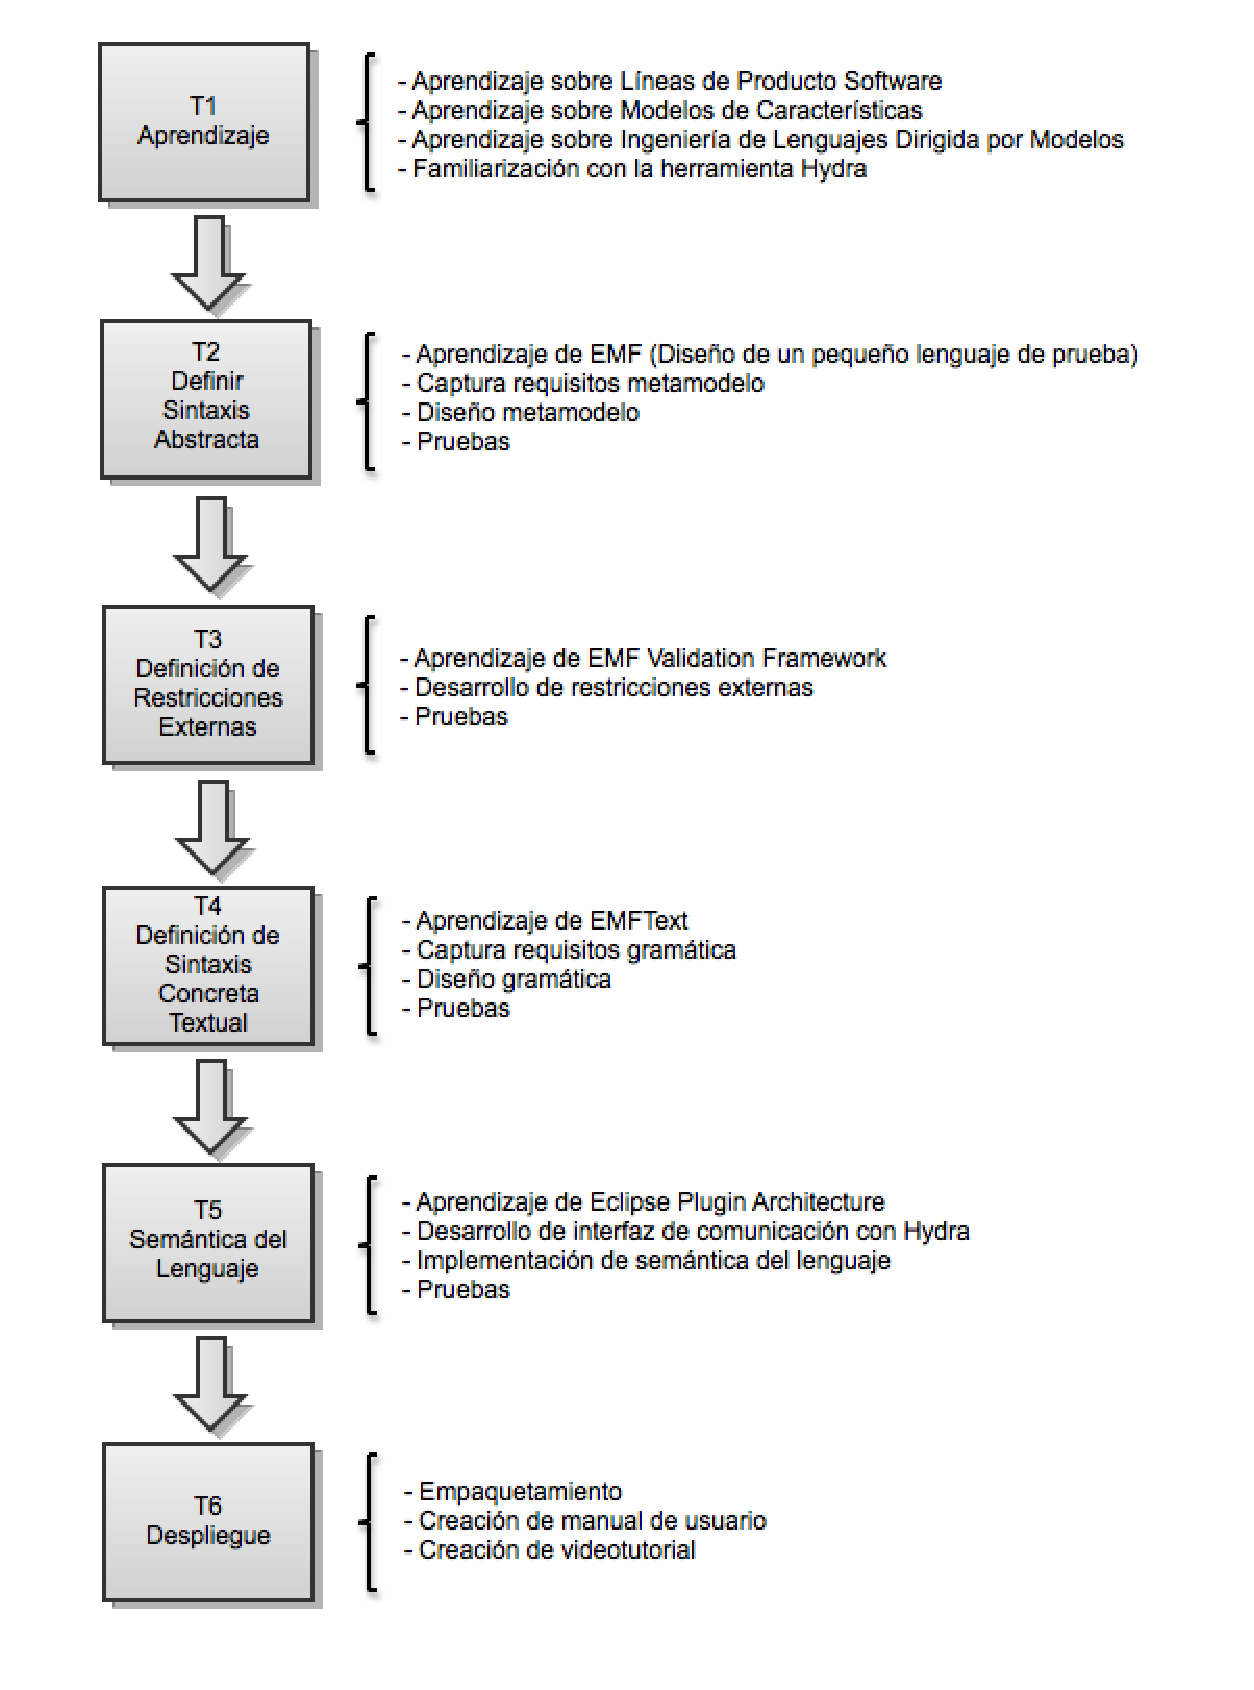
\includegraphics[scale=0.74]{planificacion/planning.eps}
    \caption{Proceso de desarrollo del Proyecto Fin de Carrera}
    \label{fig:planning}
\end{figure}

Obviamente, la primera tarea (Figura~\ref{fig:planning}-\emph{T1}) en este proceso de desarrollo fue la de adquirir los conocimientos necesarios para la realizaci�n de todas las tareas posteriores. Ello implicaba adquirir los conocimientos relacionados con las \emph{L�neas de Producto Software}~\cite{} en general y con los �rboles de caracter�sticas~\cite{} en particular, m�s concretamente, con la vesi�n de los �rboles de caracter�sticas que soportan la definici�n de caracter�sticas clonables~\cite{}. Dado que el proyecto se deb�a integrar con una herramienta para la especificaci�n y configuraci�n de �rboles de caracter�sticas concreta, denominada \emph{Hydra}~\cite{}, el siguiente paso fue el de familiarizarse con dicha herramienta y adquirir ciertos conocimientos sobre su arquitectura interna.

A continuaci�n, se tuvo que adquirir los conceptos necesarios para entender el funcionamiento de de la \emph{Ingenier�a de Lenguajes Dirigida por Modelos}~\cite{}. La familiarizaci�n con las tecnolog�as concretas relacionadas con la \emph{Ingenier�a de Lenguajes Dirigida por Modelos}, como la utilizaci�n de EMF (\emph{Eclipse Modelling Framework})~\cite{} para la definici�n de metamodelos, se realiz� dentro de cada fase concreto del proyecto, a medida que se iba necesitando aprender a utilizar dichas tecnolog�as.

%%========================================================================================%%
%% NOTA(Pablo): No pongas los tiempos que te ha costado cada tarea. Normalmente, no
%%              interesa y da mala imagen
%%========================================================================================%%

Tras esta tarea inicial de adquisici�n de conocimientos previos, el resto del proyecto se estructura como un proyecto de desarrollo de un lenguaje software siguiendo un enfoque dirigido por modelos. Consecuentemente, la primera tarea tras la fase inicial de documentaci�n (Figura~\ref{fig:planning}-\emph{T2}) fue la definici�n de la sintaxis abstracta, por medio de un metamodelo m�s un conjunto de restricciones externas, para el lenguaje que deb�a soportar nuestro editor. Para ello tuvimos que capturar los requisitos que deb�a satisfacer dicho lenguaje. Tras recoger dichos requisitos, se procedi� al dise�o del metamodelo y a la relizaci�n de las pruebas pertinentes con vistas a comprobar su correcto funcionamiento. Para crear dicho metamodelo se utiliz� el lenguaje de metamodelado Ecore, integrado dentro de la herramienta EMF (Eclipse Modelling Framework)~\cite{}.

A continuaci�n, de acuerdo con los expuesto en la secci�n anterior, procedimos a definir la las restricciones externas que no pod�an ser definidas en Ecore (Figura~\ref{fig:planning}-\emph{T3}). Dichas restricciones se implementaron utilizando la facilidad de EMF denominada EMF Validation Framework~\cite{}.

A continuaci�n, procedimos a definir la sintaxis concreta, en nuestro caso textual, para nuestro lenguaje de modelado. Optamos por una sintaxis textual ya que las restricciones a especificar son una especie de f�rmulas l�gicas, las cuales resultan m�s c�modas de especificar mediante notaciones textuales que mediante notaciones gr�ficas (Figura~\ref{fig:planning}-\emph{T4}). Para el desarrollo de dicha sintaxis textual hubo que hacer un nuevo an�lisis de los requisitos que dicha notaci�n textual deb�a satisfacer. A continuaci�n se especific� la gram�tica de nuestra sintaxis textual, ligando sus elementos con los del metamodelo producido en la fase anterior y se ejecutaron los casos de prueba necesarios para comprobar su correcto funcionamiento. Para crear dicha sintaxis textual se utiliz� la herramienta EMFText~\cite{}.

Las etapas anteriores permit�an disponer de un editor que soportaba la especificaci�n de restricciones de acuerdo al lenguaje HCL. Por tanto, s�lo restaba poder comprobar, para una configuraci�n dada de un �rbol de caracter�sticas, que dichas restricciones se satisfac�an. Ello implicaba dotar de sem�ntica al lenguaje y, a partir de dicha sem�ntica, implementar los mecanismos necesarios para la comprobaci�n de la validez de dichas restricciones. La sem�ntica del lenguaje ya estaba definida por el profesor Pablo S�nchez, por lo que s�lo hubo que implementar el c�digo necesario para procesar un modelo de restricciones y comprobar que dichas restricciones se satisfac�an. Dicho c�digo se implement� en Java, utilizando las facilidades que el entorno EMF proporciona para la manipulaci�n del modelo  (Figura~\ref{fig:planning}-\emph{T5}). Para poder implementar la sem�ntica, fue necesario crear una interfaz de comunicaci�n con la herramienta \emph{Hydra} que permitiese conocer el estado en el cual se hallaba cada caracter�stica. Tras la implementaci�n, se ejecut� un exhaustivo conjunto de pruebas para comprobar el correcto funcionamiento del c�digo creado.

En este punto del proceso de desarrollo ten�amos implementado el editor requerido, por lo que s�lo restaba proceder a su despliegue (Figura~\ref{fig:planning}-\emph{T6}). Este despliegue implicaba su integraci�n dentro de la arquitectura de plugins de Eclipse y, m�s concretamente, de la herramienta \emph{Hydra}. Tras dicha integraci�n, se procedi� a realizar una serie de pruebas de aceptaci�n, destinadas a comprobar que el trabajo realizado satisfac�a las necesidades de los usuarios finales que iban a utilizar el editor creado.



\section{Estructura del Documento}
\label{sec:intr:estructura}

% %%==================================================================%%
%% Author : Tejedo Gonz�lez, Daniel                                 %%
%%          S�nchez Barreiro, Pablo                                 %%
%% Version: 1.0, 22/11/2012                                         %%
%% Version: 2.0, 31/01/2013                                         %%
%%                                                                  %%
%% Memoria del Proyecto Fin de Carrera                              %%
%% Planificacion, planificacion                                     %%
%%==================================================================%%

Como se ha comentado con anterioridad, el objetivo de este Proyecto Fin de Carrera es el desarrollo de un editor para un novedoso lenguaje de especificaci�n y validaci�n de restricciones para �rboles de caracter�sticas donde dichas restricciones puedan incluir caracter�sticas clonables. Dicho editor se desarrollar� utilizando un moderno enfoque de \emph{Ingenier�a de Lenguajes Dirigido por Modelos}. Por tanto, el proceso de desarrollo del presente proyecto queda pr�cticamente determinado por dicho enfoque, el cual posee un proceso de desarrollo bien definido, el cual se describi� en la secci�n anterior. La Figura~\ref{fig:planning} muestra como dicho proceso de desarrollo se ha instanciado para nuestro caso particular.

%%==================================================================%%
%% NOTA(Pablo): En esta imagen hay que hacer cambios                %%
%%              Te los indico de foma verbal cuando pases por el    %%
%%              despacho, pero hay que mejorar su consistencia      %%
%%==================================================================%%

\begin{figure}[!tb]
    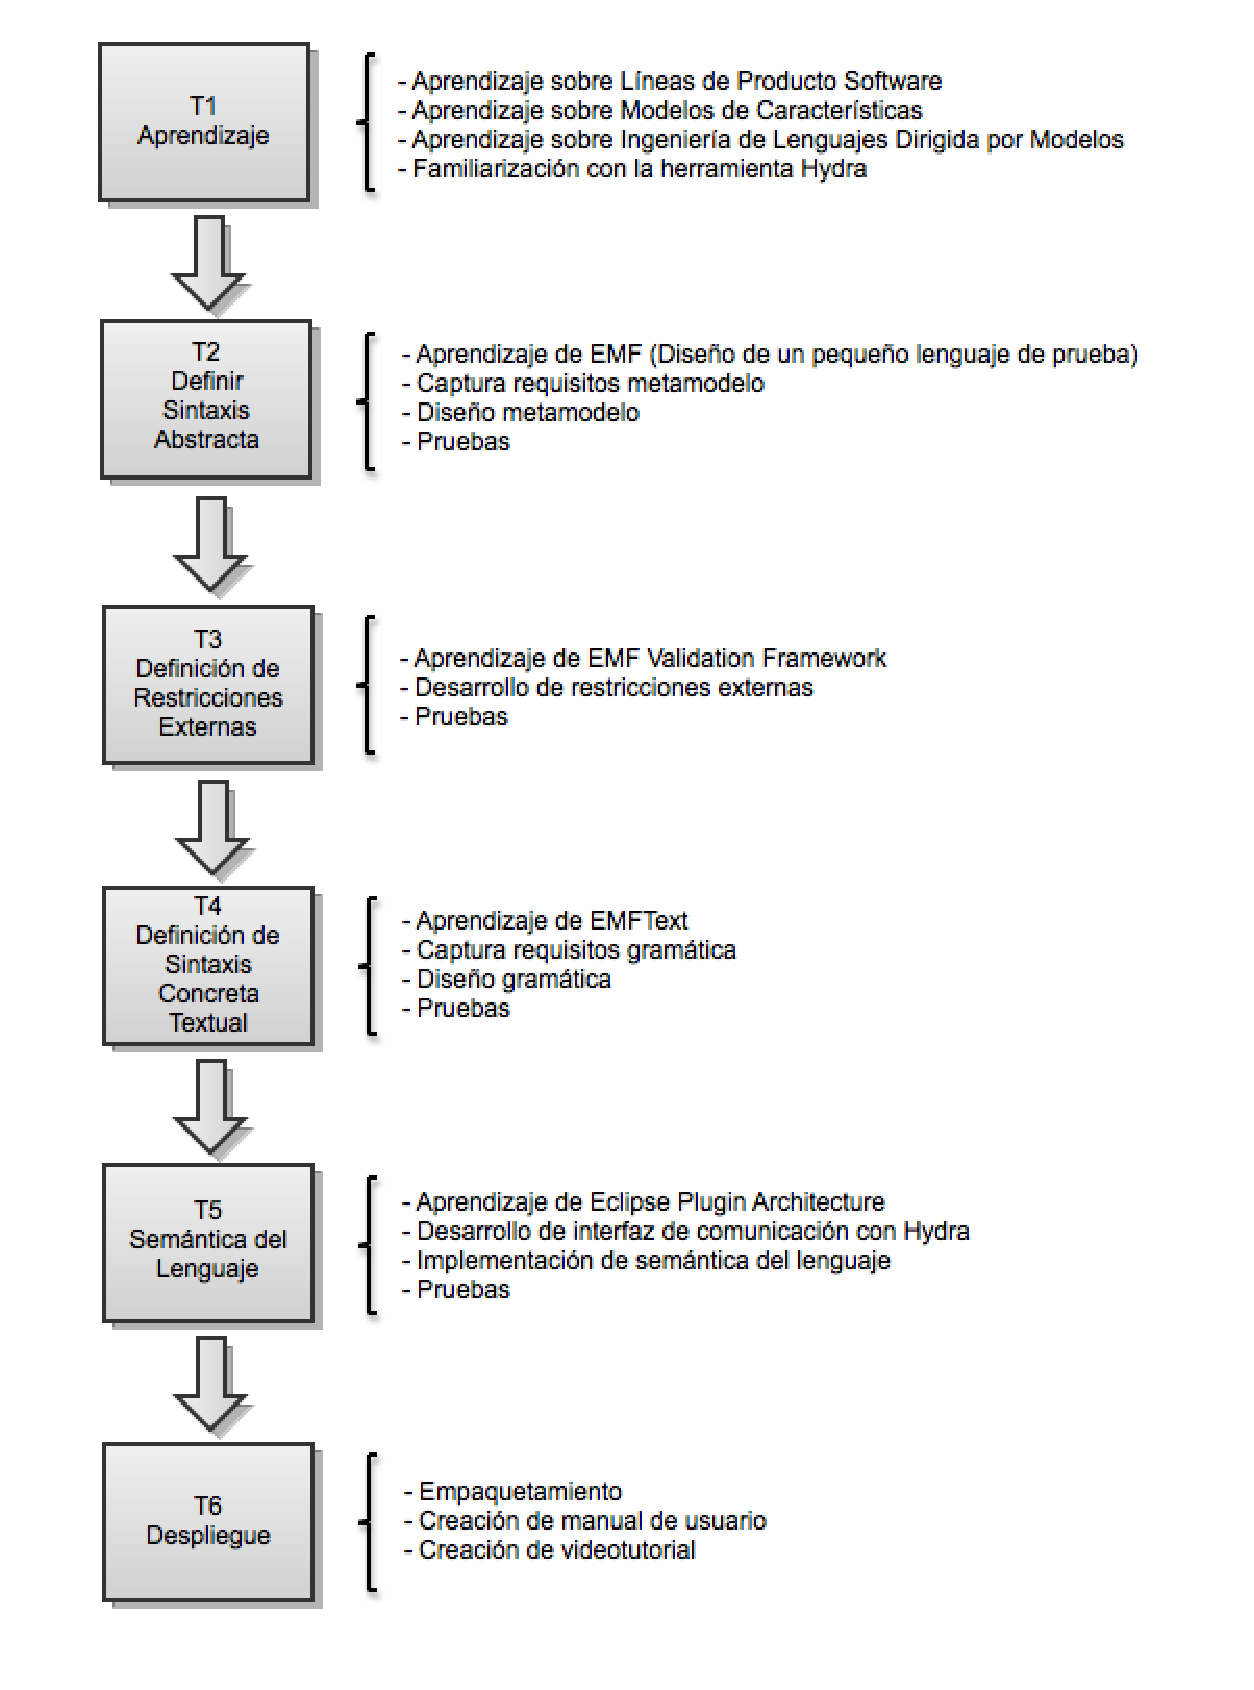
\includegraphics[scale=0.74]{planificacion/planning.eps}
    \caption{Proceso de desarrollo del Proyecto Fin de Carrera}
    \label{fig:planning}
\end{figure}

Obviamente, la primera tarea (Figura~\ref{fig:planning}-\emph{T1}) en este proceso de desarrollo fue la de adquirir los conocimientos necesarios para la realizaci�n de todas las tareas posteriores. Ello implicaba adquirir los conocimientos relacionados con las \emph{L�neas de Producto Software}~\cite{} en general y con los �rboles de caracter�sticas~\cite{} en particular, m�s concretamente, con la vesi�n de los �rboles de caracter�sticas que soportan la definici�n de caracter�sticas clonables~\cite{}. Dado que el proyecto se deb�a integrar con una herramienta para la especificaci�n y configuraci�n de �rboles de caracter�sticas concreta, denominada \emph{Hydra}~\cite{}, el siguiente paso fue el de familiarizarse con dicha herramienta y adquirir ciertos conocimientos sobre su arquitectura interna.

A continuaci�n, se tuvo que adquirir los conceptos necesarios para entender el funcionamiento de de la \emph{Ingenier�a de Lenguajes Dirigida por Modelos}~\cite{}. La familiarizaci�n con las tecnolog�as concretas relacionadas con la \emph{Ingenier�a de Lenguajes Dirigida por Modelos}, como la utilizaci�n de EMF (\emph{Eclipse Modelling Framework})~\cite{} para la definici�n de metamodelos, se realiz� dentro de cada fase concreto del proyecto, a medida que se iba necesitando aprender a utilizar dichas tecnolog�as.

%%========================================================================================%%
%% NOTA(Pablo): No pongas los tiempos que te ha costado cada tarea. Normalmente, no
%%              interesa y da mala imagen
%%========================================================================================%%

Tras esta tarea inicial de adquisici�n de conocimientos previos, el resto del proyecto se estructura como un proyecto de desarrollo de un lenguaje software siguiendo un enfoque dirigido por modelos. Consecuentemente, la primera tarea tras la fase inicial de documentaci�n (Figura~\ref{fig:planning}-\emph{T2}) fue la definici�n de la sintaxis abstracta, por medio de un metamodelo m�s un conjunto de restricciones externas, para el lenguaje que deb�a soportar nuestro editor. Para ello tuvimos que capturar los requisitos que deb�a satisfacer dicho lenguaje. Tras recoger dichos requisitos, se procedi� al dise�o del metamodelo y a la relizaci�n de las pruebas pertinentes con vistas a comprobar su correcto funcionamiento. Para crear dicho metamodelo se utiliz� el lenguaje de metamodelado Ecore, integrado dentro de la herramienta EMF (Eclipse Modelling Framework)~\cite{}.

A continuaci�n, de acuerdo con los expuesto en la secci�n anterior, procedimos a definir la las restricciones externas que no pod�an ser definidas en Ecore (Figura~\ref{fig:planning}-\emph{T3}). Dichas restricciones se implementaron utilizando la facilidad de EMF denominada EMF Validation Framework~\cite{}.

A continuaci�n, procedimos a definir la sintaxis concreta, en nuestro caso textual, para nuestro lenguaje de modelado. Optamos por una sintaxis textual ya que las restricciones a especificar son una especie de f�rmulas l�gicas, las cuales resultan m�s c�modas de especificar mediante notaciones textuales que mediante notaciones gr�ficas (Figura~\ref{fig:planning}-\emph{T4}). Para el desarrollo de dicha sintaxis textual hubo que hacer un nuevo an�lisis de los requisitos que dicha notaci�n textual deb�a satisfacer. A continuaci�n se especific� la gram�tica de nuestra sintaxis textual, ligando sus elementos con los del metamodelo producido en la fase anterior y se ejecutaron los casos de prueba necesarios para comprobar su correcto funcionamiento. Para crear dicha sintaxis textual se utiliz� la herramienta EMFText~\cite{}.

Las etapas anteriores permit�an disponer de un editor que soportaba la especificaci�n de restricciones de acuerdo al lenguaje HCL. Por tanto, s�lo restaba poder comprobar, para una configuraci�n dada de un �rbol de caracter�sticas, que dichas restricciones se satisfac�an. Ello implicaba dotar de sem�ntica al lenguaje y, a partir de dicha sem�ntica, implementar los mecanismos necesarios para la comprobaci�n de la validez de dichas restricciones. La sem�ntica del lenguaje ya estaba definida por el profesor Pablo S�nchez, por lo que s�lo hubo que implementar el c�digo necesario para procesar un modelo de restricciones y comprobar que dichas restricciones se satisfac�an. Dicho c�digo se implement� en Java, utilizando las facilidades que el entorno EMF proporciona para la manipulaci�n del modelo  (Figura~\ref{fig:planning}-\emph{T5}). Para poder implementar la sem�ntica, fue necesario crear una interfaz de comunicaci�n con la herramienta \emph{Hydra} que permitiese conocer el estado en el cual se hallaba cada caracter�stica. Tras la implementaci�n, se ejecut� un exhaustivo conjunto de pruebas para comprobar el correcto funcionamiento del c�digo creado.

En este punto del proceso de desarrollo ten�amos implementado el editor requerido, por lo que s�lo restaba proceder a su despliegue (Figura~\ref{fig:planning}-\emph{T6}). Este despliegue implicaba su integraci�n dentro de la arquitectura de plugins de Eclipse y, m�s concretamente, de la herramienta \emph{Hydra}. Tras dicha integraci�n, se procedi� a realizar una serie de pruebas de aceptaci�n, destinadas a comprobar que el trabajo realizado satisfac�a las necesidades de los usuarios finales que iban a utilizar el editor creado.






\section{Metamodelo Cassandra}
\label{domain:sec:metamodelo}
%%==========================================================================%%
%% Author : Sa�udo Olmedo, Ignacio                                          %%
%% Author : S�nchez Barreiro, Pablo                                         %%
%% Version: 1.2, 23/04/2014                                                 %%
%%                                                                          %%
%% Memoria del Proyecto Fin de Carrera                                      %%
%% M2M/MetamodeloCassandra                                                  %%
%%==========================================================================%%

Previo paso a la definici�n de las reglas de transformaci�n entre modelos necesitamos definir un meta-modelo de origen y un meta-modelo de destino. Como hab�amos descrito en el capitulo anterior la base del proceso de transformaci�n entre modelos parte del meta-modelo. El meta-modelo de UML 2.0 utilizado en este proyecto como origen de la transformaci�n es el que nos proporciona Epsilon, dicho meta-modelo sigue el est�ndar de UML 2.0. A parte del meta-modelo de UML nos hace falta un meta-modelo que defina el lenguaje de modelado de Cassandra. Dicho meta-modelo fue proporcionado por Pablo S�nchez Barreiro. Este meta-modelo se construyo por medio de la abstracci�n de las principales caracter�sticas de Cassandra. El meta-modelo sufri� algunos cambios respecto al inicial debido a exigencias y variantes que sufri� el proyecto. La Figura~\ref{back:fig:metamodeloCassandra} muestra un diagrama de clase UML que representa el modelo de datos de Cassandra. Este tipo de modelo es el origen del proceso de transformaciones entre modelos que queremos crear. A continuaci�n se detallan los aspectos m�s importantes del meta-modelo de Cassandra.

\begin{figure}[!tb]
  \centering
  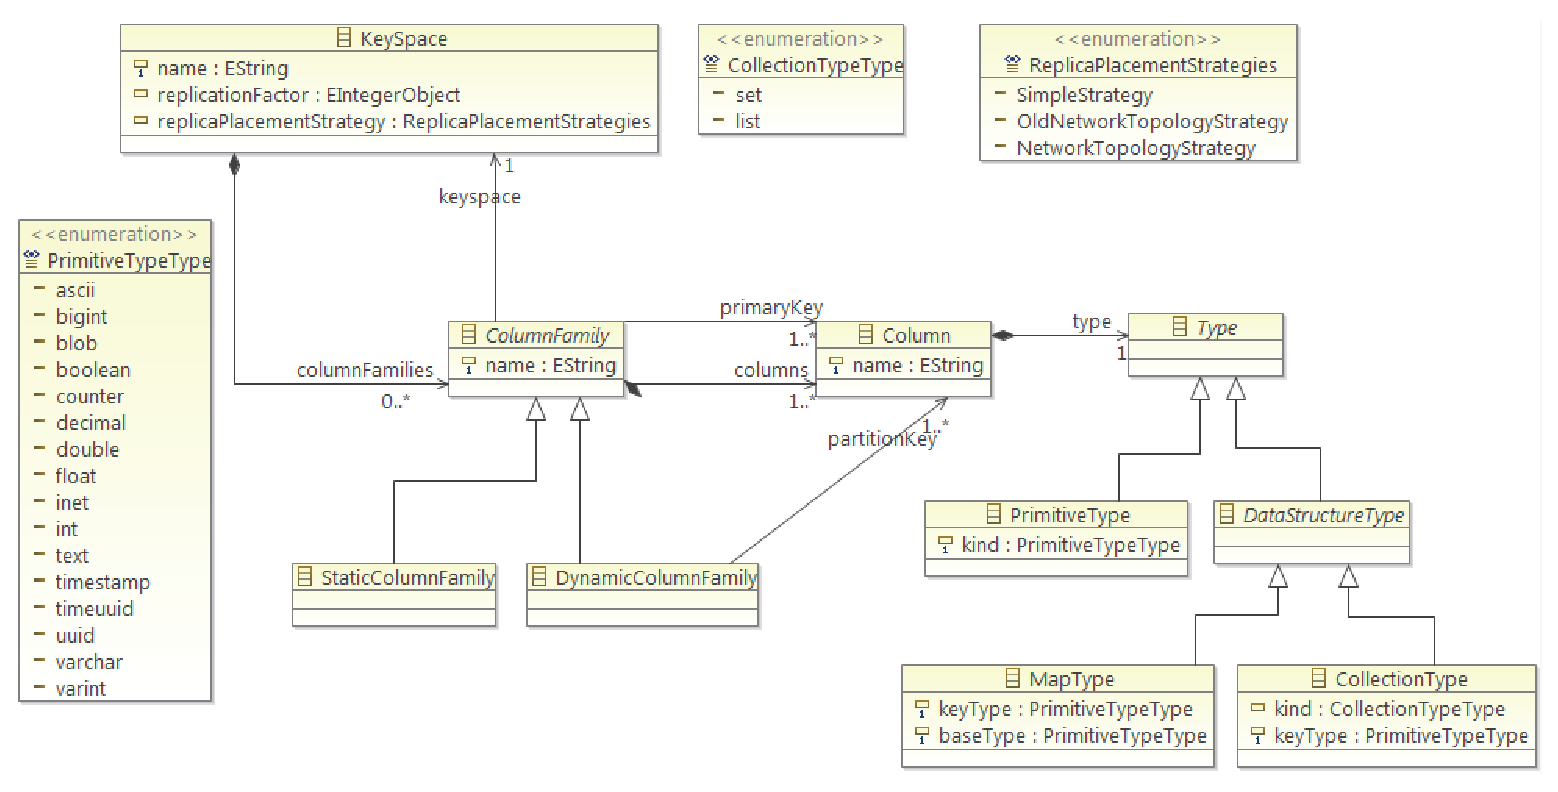
\includegraphics[width=.8\linewidth]{m2m/images/ecoreDiag.eps} \\
  \caption{Metamodelo Cassandra}
  \label{back:fig:metamodeloCassandra}
\end{figure}

De acuerdo con la arquitectura de Cassandra, el elemento ra�z de cualquier esquema orientado a columnas es el keyspace, el keyspace es el equivalente a la base de datos en el modelo relacional, la meta-clase keyspace cuenta con los meta-atributos: nombre utilizado para denominar el keyspace, [cassandra] replicationFactor que representa el n�mero de servidores de Cassandra de los que se debe guardar un registro u obtener una respuesta al recuperar alg�n registro y replicaPlacementStrategy es la estrategia de replicaci�n que se va a tomar, dentro de estas estrategias de replicaci�n encontramos tres tipos: %[http://www.datastax.com/docs/1.0/cluster_architecture/replication]:

\begin{enumerate}
\item SimpleStrategy: Es la estrategia de replicaci�n utilizada por defecto al crear un keyspace utilizando Cassandra. Es utilizada para cl�steres de datacenters simples.
\item NetworkTopologyStrategy: Utilizada cuando el cl�ster es desplegado a trav�s de m�ltiples data centers. Esta estrategia especifica cu�ntas r�plicas se desean en cada data center.
\item OldNetworkTopologyStrategy: Se utiliza para proporcionar retro-compatibilidad con instalaciones de Cassandra antiguas.
\end{enumerate}

A continuaci�n tenemos la meta-clase ColumnFamily equivalente a las tablas en el modelo relacional, dentro de esta meta-clase encontramos dos tipos: las StaticColumnFamily y las DynamicColumnFamily. Recordamos que las static column family son el equivalente a las tablas en el modelo relacional, sin embargo las dynamic column family son utilizadas para la recuperaci�n de datos eficiente, algo similar a las vistas del modelo relacional. %[http://www.datastax.com/docs/1.1/ddl/column_family#dynamic-column-families].

En cuanto a la definici�n de la primary key, las column families est�ticas siguen una definici�n de claves cl�sica por lo que en el meta-modelo no se refleja, sin embargo las column families din�micas tienen una definici�n de la primary key especial. A la hora de definir esta primary key hay que tener en cuenta el orden, en CQL el orden de definici�n de las claves importa, en la primera columna de la primary key se define la partition key, esta tiene la propiedad de que todas las filas que comparten la misma partition key se almacenan en el mismo nodo f�sico. %[http://www.datastax.com/docs/1.1/ddl/indexes].
Adem�s, la inserci�n, actualizaci�n o eliminaci�n de filas que comparten la partition key para una column family determinada se realizan de forma at�mica. Es posible tener una partition key compuesta, es decir, una partition key formada por varias columnas, en CQL esto se define utilizando par�ntesis para delimitar el conjunto de partici�n. En la siguiente columna se define la clustering key utilizada para la recuperaci�n de filas de manera eficiente. En el meta-modelo solo tendremos en cuenta las partition key puesto que las columnas que no son definidas como partition key se toman como cluster key.
Aunque en siguientes secciones esta informaci�n se amplia, el resumen de la definici�n de column families din�micas es la siguiente: PRIMARY KEY((partitioning key\_1, ... partitioning key\_n), clustering key\_1 ... clustering key\_n)


La siguiente meta-clase es Column, esta meta-clase contiene los valores que se almacenan en las column families, estas columns tienen como meta-atributos el nombre y un tipo de dato.
Dentro de los tipos de datos que pueden darse en una columna encontramos dos meta-tipos, PrimitiveType y DataStructureType.
PrimitiveType define los tipos primitivos, por ejemplo entero, texto, uuid, etc..
DataStructureType define las colecciones. Estas colecciones pueden ser de dos tipos: MapType o bien CollectionType, ambas colecciones tienen un meta-atributo llamado KeyType para definir el tipo primitivo que utilizan. MapType cuenta con un meta-atributo llamado baseType de tipo primitivo que define el segundo tipo de dato del mapa. Dentro de CollectionType encontramos un meta-atributo llamado kind que define el tipo de colecci�n que vamos a utilizar, esta puede ser o bien tipo set o tipo list. M�s adelante se explica que caracter�sticas re�ne cada colecci�n y mapa y cuando se utilizan.


\section{Transformaci�n de Modelo UML a Cassandra}
\label{domain:sec:transformation}
%%==================================================================%%
%% Author : Sa�udo Olmedo, Ignacio                                  %%
%% Author : S�nchez Barreiro, Pablo                                 %%
%% Version: 1.4, 29/04/2014                                         %%
%%                                                                  %%
%% Memoria del Proyecto Fin de Carrera                              %%
%% M2M/Reglas Transformaci�n UML a Cassandra                        %%
%%==================================================================%%

Una vez definido el meta-modelo de Cassandra podemos establecer las reglas de transformaci�n entre modelos UML y modelos Cassandra, para ello utilizaremos Epsilon Transformation Language (ETL). Recordamos que el lenguaje ETL es el lenguaje que utiliza Epsilon para la transformaci�n entre modelos basado en reglas.
Las reglas de transformaci�n son definidas en [docPablo]. A continuaci�n se detalla c�mo se han implementado dichas reglas.

\subsection{Transformaci�n del modelo}
El modelo UML se considera el elemento ra�z que contiene como es evidente, todos los elementos del modelo, este modelo de datos se transforma en el keyspace para el repositorio de Cassandra. El nombre del keyspace corresponder� al que se haya escogido para el modelo de datos UML. Los Key Spaces permiten agrupar entidades tales como Column Families, Columns.. De esta forma, se pueden tener varios Key Spaces en el mismo proyecto independientes entre s�.

\subsection{Transformaci�n de clases}
Se han definido dos reglas ETL que transforman una clase definida en UML a una static column family de Cassandra (el equivalente a una tabla en el sistema de bases de datos relacionales).
La primera regla es definida para las clases que tengan un atributo clave definido, para ello se utiliza la propiedad isID de UML la cual define que ese atributo identifica a la clase de forma �nica. La segunda regla es para las clases sin atributo clave definido. El proceso de transformaci�n es similar en ambas reglas, en primer lugar se transforma la clase UML a una column family de Cassandra, se asigna la column family al keyspace que le corresponde, se copia el nombre de la clase a la column family y se a�ade al conjunto de column families del keyspace. La segunda regla es utilizada para las clases sin atributo clave, en este caso se crea un atributo que va a ser la clave de esa column family (ya que esta no tiene), dicha clave tendr� de nombre, el nombre de la clase m�s el distintivo \_ID y ser� de tipo uuid.
Dichas reglas est�n definidas en el punto 5.3 del documento [docPablo].

\subsection{Transformaci�n de atributos}
La siguiente regla define como se realiza la transformaci�n de un atributo del modelo UML a una columna del modelo Cassandra. La definici�n b�sica es que un atributo UML corresponde a una columna Cassandra. Para ello en primer lugar se define una guarda ETL para que la transformaci�n se haga solo de los atributos de las clases y no de los atributos de la relaci�n ya que al importar los modelos UML existen atributos ajenos al modelo de datos que son importados a Epsilon. A continuaci�n se realiza un filtro para evitar la adici�n de columnas que no pertenezcan al modelo de datos. Una vez hecho esto hay que diferenciar dos tipos de atributos, aquellos cuya multiplicidad sea igual a 1 y aquellos atributos con multiplicidad mayor de 1.
En cuanto a los atributos de multiplicidad igual a 1 se realiza la transformaci�n del atributo a columna copiando su tipo de dato.
Respecto a los atributos de tama�o mayor de 1 se aplica la siguiente regla: Aquellos atributos que se hayan definido en el modelo UML como �nicos y no ordenados son transformados como tipo set de Cassandra. En caso contrario se definen como tipo list.
Una vez transformado el atributo en un set o en una list, en ambos casos se realiza la transformaci�n correspondiente del tipo primitivo UML a Cassandra (viene descrita en la �ltima sub-secci�n), se realiza una copia del nombre y se a�ade la columna ya transformada a la column family correspondiente.
Finalmente en caso de que el atributo sea clave de la clase se a�ade a la column family como primary key. El c�digo correspondiente a esta regla es el que se puede observar en la figura~\ref{back:code:reglaTrans}

\begin{figure}[!tb]
\begin{center}
\begin{footnotesize}
\begin{verbatim}
--------------------------------------------------------
//5.5 Attribute with primitive type transformation
rule Attribute2Column
transform attribute : UML!Property
to column : nosql!Column {
    guard: ((""+attribute.qualifiedName).contains("Data::") and attribute.type.isKindOf(UML!PrimitiveType))

    //filtramos para evitar a�adir columnas ajenas al modelo de datos
    for(cfamily in kspace.columnFamilies){	

        if(attribute.qualifiedName=="Data::"+cfamily.name+"::"+attribute.name){

            //5.5 Attribute with primitive type transformation->Attributes with upper bound = 1
            if(attribute.upper=1){
                //transformacion del atributo en una columna basica
                var type : new nosql!PrimitiveType;
                type.kind=umlType2modelType(attribute.type.name);
                column.type=type;
            }
            //5.5 Attribute with primitive type transformation->Attributes with upper bound > 1
            else if(attribute.upper<>0){
                //transformacion del atributo en un set o list
                var ctype : new nosql!CollectionType;

                if(attribute.isUnique and not attribute.isOrdered)//set
                    ctype.kind=nosql!CollectionTypeType#set;
                else//list
                    ctype.kind=nosql!CollectionTypeType#list;

                ctype.keyType=umlType2modelType(attribute.type.name);
                column.type=ctype;
            }

            column.name=attribute.name;			
            cfamily.columns.add(column);		

            //5.1 Assignment of keys to classes
            if(attribute.isID)
                cfamily.primaryKey.add(column);
        }
    }
}
--------------------------------------------------------
\end{verbatim}
\end{footnotesize}
\end{center}
\caption{Regla de transformaci�n XX}
\label{back:code:reglaTrans}
\end{figure}

\subsection{Transformaci�n de asociaciones}
La siguiente regla define como se realiza la transformaci�n de los atributos de las asociaciones entre clases UML.
En primer lugar hay que diferenciar como se tratan las asociaciones, existen dos tipos de asociaciones: aquellas asociaciones cuyo extremo tiene una cardinalidad igual a uno y aquellas con una cardinalidad mayor de uno.

Para los extremos con cardinalidad igual a uno se crea una columna que ser� a�adida en la column family del otro extremo de la relaci�n, esta columna nueva es una copia de la columna que es primary key en la column family fuente, el nombre de la nueva columna es la composici�n del nombre de la column family y del nombre de la primary key, el tipo de la nueva columna es el mismo que el de la columna primary key de la column family fuente. Esto se comprende mejor con el caso de estudio propuesto en la secci�n siguiente.

Para los extremos con cardinalidad mayor de uno, se crea una dynamic column family. Recordamos que la primary key de este tipo de column family esta compuesta de dos tipos de columnas: La partition key y la cluster key.
La transformaci�n utilizada para este tipo de column family es la siguiente: Esta column family din�mica est� compuesta de dos columnas, la primera columna juega el papel de partition key y la segunda columna de cluster key, la primera columna se construye de la misma manera que el caso anterior, se copia el nombre y el tipo de la primary key de la column family extremo de la asociaci�n fuente. La segunda columna de la misma manera toma los datos nombre y tipo de la primary key del otro extremo de la asociaci�n. 
El nombre de la column family ser� la concatenaci�n del nombre de las column family de ambos extremos de la asociaci�n (primero fuente, segundo extremo fin de la asociaci�n).
En resumen la transformaci�n de la primary key en las column family din�micas es la siguiente:
\begin{enumerate}
\item Partition Key: Primera columna  (fuente de la asociaci�n).
\item Clustering Key: Segunda columna (extremo de la asociaci�n).
\end{enumerate}
	
\subsection{Transformaci�n de tipos primitivos}
En cuanto a la transformaci�n de variables de tipo primitivo se define una operaci�n b�sica de correspondencia entre tipos, de esta manera podemos convertir un tipo primitivo UML a su equivalente en Cassandra. Las correspondencias definidas ser�an las siguientes:

\begin{table}[!hbt]
\begin{center}
\begin{tabular}{||l | c | r||}
\hline
\hline
\textbf{UML} & \textbf{Cassandra} \\
\hline
string & text \\
\hline
int & int \\
\hline
date & timestamp \\
\hline
uuid & uuid \\
\hline
float & float \\
\hline
double & double \\
\hline
boolean & boolean \\
\hline
char & varchar \\
\hline
\end{tabular}
\caption{Equivalencias tipos primitivos UML-Cassandra}
\end{center}
\end{table}




\section{Caso de estudio transformaci�n modelo a modelo}
\label{domain:sec:casoEstudio}
%%==========================================================================%%
%% Author : Sa�udo Olmedo, Ignacio                                          %%
%% Author : S�nchez Barreiro, Pablo                                         %%
%% Version: 1.2, 21/04/2014                                                 %%
%%                                                                          %%
%% Memoria del Proyecto Fin de Carrera                                      %%
%% M2M/Caso de estudio                                                      %%
%%==========================================================================%%

Como se explicaba en el capitulo 2 en la secci�n "Caso de estudio" el objetivo de este caso de estudio es la creaci�n de un generador de c�digo de una versi�n simplificada de Twitter.
En esta secci�n se reproducir�n los procesos M2M y M2T en el siguiente capitulo, todo esto bajo el proceso de desarrollo dirigido por modelos. Esta secci�n esta dedicada a describir la transformaci�n del modelo UML de Twissandra a un modelo Cassandra. Partiendo del modelo UML de la figura~\ref{back:fig:twissandra} y una vez establecidas las reglas de transformaci�n entre modelos, esta secci�n explica el proceso de transformaci�n del modelo UML al modelo Cassandra.

En primer lugar, marcamos el atributo username de la clase User como clave. En el caso de la clase FollowingRelationship y la clase Tweet al no tener un atributo marcado como clave generamos una clave sustituta autom�ticamente para cada clase, llamadas FollowingRelationship\_id y tweet\_id respectivamente.

Por cada paquete estereotipado como <<dataModel>>, se crea un nuevo keyspace. El nombre del keyspace ser� el nombre utilizado por el data model. Los atributos restantes de las meta-clases del keyspace se establecen en sus valores definidos por defecto. A continuaci�n, todos los elementos correspondientes de ese paquete se procesan y se colocan dentro de su keyspace correspondiente.

Como se mencionaba en las reglas de transformaci�n, la clase User se transforma en una Column Family llamada User. A continuaci�n, los atributos y las asociaciones se procesan. Por �ltimo, el atributo Username, que se marc� como clave en el modelo de datos UML, es marcado como Primary Key. De manera similar para aquellos atributos del modelo UML cuya multiplicidad sea igual a uno se realiza una transformaci�n simple, por ejemplo el atributo username y password se transforman en dos columnas, ambos del tipo text. Estas columnas est�n contenidas en la column family User. De la misma manera se transforman los atributos body y time de la clase Tweet y el atributo timestamp de la clase FollowingRelationship.
En el caso de el atributo del modelo UML email cuya multiplicidad es mayor de uno y tiene las propiedades isUnique establecida en false y la propiedad isOrdered establecida en false (en el modelo no se puede apreciar pero esta configurado as�), se transforma este atributo en un set llamado email de tipo text dentro de la column family User.

En cuanto a las asociaciaciones de multiplicidad igual a uno la transformaci�n que se realiza por ejemplo, para la asociaci�n de la clase user una nueva columna llamada user\_username (recordemos que username es la clave de la column family user) es creada y a�adida a la column family Tweet. Para las asociaciones cuya multiplicidad es mayor de uno, por ejemplo la asociaci�n llamada userline se crea una dynamic column family llamada User\_userline. A continuaci�n una columna llamada user\_username de tipo text es a�adida a esta column family. Despu�s una columna llamada tweet\_id de tipo uuid es a�adida (el atributo tweet\_id fue creado en la column family tweet al no tener clave). Las columnas user\_username y tweet\_id son designadas como primary key, la columna user\_username ser� la partition key. 

\section{Sumario}
\label{domain:sec:sumario}
%%==================================================================%%
%% Author : Abascal Fern�ndez, Patricia                             %%
%%          S�nchez Barreiro, Pablo                                 %%
%% Version: 1.1, 21/06/2013                                         %%
%%                                                                  %%
%% Memoria del Proyecto Fin de Carrera                              %%
%% Antecedentes, Sumario                                            %%
%%==================================================================%%

Durante este cap�tulo se han descrito los conceptos necesarios para comprender el �mbito y el alcance de este proyecto. Se ha descrito el caso de estudio que se utilizar� a lo largo del documento. A continuaci�n, se ha especificado qu� es una l�nea de productos software, el dise�o orientado a caracter�sticas, la metodolog�a TENTE, las limitaciones de las clases parciales en C\#, c�mo pueden resolverse estas limitaciones mediante el uso del \emph{SlicerPattern} y el proceso de generaci�n de c�digo con Epsilon.




% Cap�tulo 4: Application Engineering
% %%==================================================================%%
%% Author : Sa�udo Olmedo, Ignacio                                  %%
%% Author : S�nchez Barreiro, Pablo                                 %%
%% Version: 1.2, 15/05/2014                                         %%
%%                                                                  %%
%% Memoria del Proyecto Fin de Carrera                              %%
%% Cap�tulo m2t, Archivo ra�z                                       %%
%%==================================================================%%

\chapterheader{Manual}{Manual}
\label{chap:manual}


\chaptertoc

\section{Sumario}
\label{manual:sec:sumario}
%%==================================================================%%
%% Author : Abascal Fern�ndez, Patricia                             %%
%%          S�nchez Barreiro, Pablo                                 %%
%% Version: 1.1, 21/06/2013                                         %%
%%                                                                  %%
%% Memoria del Proyecto Fin de Carrera                              %%
%% Antecedentes, Sumario                                            %%
%%==================================================================%%

Durante este cap�tulo se han descrito los conceptos necesarios para comprender el �mbito y el alcance de este proyecto. Se ha descrito el caso de estudio que se utilizar� a lo largo del documento. A continuaci�n, se ha especificado qu� es una l�nea de productos software, el dise�o orientado a caracter�sticas, la metodolog�a TENTE, las limitaciones de las clases parciales en C\#, c�mo pueden resolverse estas limitaciones mediante el uso del \emph{SlicerPattern} y el proceso de generaci�n de c�digo con Epsilon.









% Cap�tulo 5: Discusi�n, Conclusiones y Trabajos Futuros
% %%==================================================================%%
%% Author : Sa�udo Olmedo, Ignacio                                  %%
%% Author : S�nchez Barreiro, Pablo                                 %%
%% Version: 1.2, 15/05/2014                                         %%
%%                                                                  %%
%% Memoria del Proyecto Fin de Carrera                              %%
%% Cap�tulo m2t, Archivo ra�z                                       %%
%%==================================================================%%

\chapterheader{Manual}{Manual}
\label{chap:manual}


\chaptertoc

\section{Sumario}
\label{manual:sec:sumario}
%%==================================================================%%
%% Author : Abascal Fern�ndez, Patricia                             %%
%%          S�nchez Barreiro, Pablo                                 %%
%% Version: 1.1, 21/06/2013                                         %%
%%                                                                  %%
%% Memoria del Proyecto Fin de Carrera                              %%
%% Antecedentes, Sumario                                            %%
%%==================================================================%%

Durante este cap�tulo se han descrito los conceptos necesarios para comprender el �mbito y el alcance de este proyecto. Se ha descrito el caso de estudio que se utilizar� a lo largo del documento. A continuaci�n, se ha especificado qu� es una l�nea de productos software, el dise�o orientado a caracter�sticas, la metodolog�a TENTE, las limitaciones de las clases parciales en C\#, c�mo pueden resolverse estas limitaciones mediante el uso del \emph{SlicerPattern} y el proceso de generaci�n de c�digo con Epsilon.









% CONTENT: Appendices, if desired
% \renewcommand\chaptername{Appendix}                      % hereafter, chapters are called "Appendix"
\renewcommand\thechapter{\Alph{chapter}}        % chapter number in Romans
\renewcommand\thesection{\Alph{chapter}.\alph{section}}  % make sections "I.a", instead of "1.1"
\setcounter{chapter}{0}                                  % start numbering chapters from 1 on again


% Appendix A:
% \input{populo/populo.tex} % Appendix I

% CONFIG: Bibliography style
\cleardoublepage                            % start in right side page
\addcontentsline{toc}{chapter}{References}  % add this "chapter" to the ToC, with the name "Bibliography"
%\bibliographystyle{alpha}                  % bibliography style
\bibliographystyle{apa}                  % bibliography style

\bibliography{references/references}

\end{document}
